\documentclass{article} 

%\usepackage{amsmath,amsthm,amsfonts}
\usepackage[bulgarian]{babel}
\usepackage[numbers]{natbib}
\usepackage{rotating}
\usepackage{amsfonts,amsmath}
\usepackage{graphicx}
\usepackage{color} 
\usepackage[notref,notcite]{showkeys}
\usepackage{multirow}
\usepackage[utf8]{inputenc}
\usepackage[T2A]{fontenc}
%\usepackage[outdir=./]{epstopdf}
\usepackage{epstopdf}
\usepackage{wrapfig}

\newcommand{\be}{\begin{equation}}
\newcommand{\ee}{\end{equation}}
\newcommand{\rf}[1]{(\ref{#1})}
\newcommand{\RR}{\mathbb{R}}
\newtheorem{thm}{Theorem}
\newtheorem{lm}{Lemma}

\newcommand{\eeth}{\rm}
\newcommand{\dO}{\partial\Omega_{h}}

\begin{document}

\section{Въведение.}\label{introduction}

Тук се разглежда двумерното уравнение на Бузинеск (УБ)
\begin{align}
&u_{tt} - \Delta u -\beta_1  \Delta u_{tt} +\beta_2 \Delta ^2 u + \Delta f(u)=0   \quad \text{for}  (x,y) \in \RR^2, \, t\in\RR^+,\label{eq1}
\\ \nonumber &u(x,y,0)=u_0(x,y), \, u_t(x,y,0)=u_1(x,y)   \quad\text{for} \, (x,y) \in \RR^2,
\\  &u(x,y) \rightarrow 0,  \Delta u(x,y) \rightarrow 0 ,  \quad \text{for}  \sqrt{x^2 + y^2} \rightarrow \infty, \label{eq11}
\end{align}
където $f(u)=\alpha u^2$, $\beta_1>0$, $\beta_2>0$ са дисперсионни параметри,  $\alpha>0$ е амплитудата, а $\Delta$ е оператора на Лаплас. Извеждането на уравнението от оригиналната система е направено в \cite{ChChr}. Целта на настоящия труд е да потърси решения на \rf{eq1} от вида $u(x,y,t)=U(x,y-ct)$, който са стационарни солитонни вълни (ССВ) движещи се по $y$ оста със скорост $c$. В последствие тези вълни ще служат за начално условие на хиперболичното (УБ) \rf{eq1} -- \rf{eq11}. Важно е да получим начално условие с добра точност чрез един гъвкав и устойчив процес, който ще позволи тестването на повече и различни сценарии. Предисторията на изчисляването на ССВ за уравнение \rf{eq1} е свързана с няколко числени техники, както следва. Спектрален метод на Галеркин е изполван в \cite{chr-chr-07,chr-chr}. Шаблони с крайни разлики от втори порядък са приложени в \cite{Ch2012}. Пертурбационно решение с развитие в ред около малък параметър (скоростта) $c$ е представено в  \cite{Ch2011}, а в последствие полученият числен резултат е апроксимиран с подходящи формули в \cite{Ch2011}. Последните алгебрични изрази са използвани като начално условие за числени симулации на нестабилното УБ \rf{eq1} -- \rf{eq11}, (виж  \cite{cher,dani}). Всички тези статии показват, че при стойности на скоростта $c<0.3$, ССВ се разсейват във формата на разширяваща се пръстеновидна вълна или избухват след кратък период от време. Вижда се, че баланса между дисперсията и нелинейността в УБ \rf{eq1} е много крехък, което изисква повече усилия при запазването му. Също така е добре известно, че в едномерния случай солитонните вълни са нестабилни за малки скорости $c$ около нулата и стабилни за по-големи скорости близки до допустимия максимум $min\{1, 1/\sqrt{\beta_1/\beta_2}\}$.
Тези наблюдения изместват фокуса към изчисляване на ССВ $U$ от \rf{eq1} с по-голяма точност и при скорости $c > 0.7$, тъй като това е от съществено значение за конструирането на началните данни при нестабилното УБ \rf{eq1}. 
След полагане на $U(x,y-ct)=u(x,y,t)$ в \rf{eq1}, ССВ удовлетворяват следното нелинейно елиптично диференциално уравнение от четвърти ред

\begin{equation}\label{eq2}
c^2 (E-\beta_1 \Delta) U_{yy} = \Delta U -\beta_2 \Delta^2 U - \Delta f(U),
\end{equation}
където $E$ е тъждествения оператор. Решението на \rf{eq2} се изчислява с помощта на стъпките описани в \cite{Ch2012,chd-chr}, но са използвани допълнителни техники, които да гарантират за по-високите изисквания, който са изложени по-горе.
Първо, за численото решение на \rf{eq2} е използвана равномерна мрежа с еднаква стъпка $h_x$ = $h_y$ = $h$ в числената област $\Omega_h$ вместо неравномерна мрежа. Решението от \rf{eq2} се използва за начално условие в хиперболичната задача \rf{eq1} и е необходима по-гъста мрежа по цялото протежение на областта през която максимумът на вълната преминава. Това дава достатъчно мотивация да се използва равномерна стъпка навсякъде в областта като в допълнение ще получим повече инфомрация по границата $\partial \Omega_h$. Числените експерименти показват, че допълнителните апроксимации върху вече съществуващо решение от елиптичната задача (напр. при неравномерна мрежа с помощта на интерполация да се получат точките в равномерна мрежа) не водят до добър резултат. Мрежата и при двете задачи трябва да е една и съща.
Второ, приложени са крайни разлики с локална апроксимация от втори $O(h^2)$, четвърти $O(h^4)$ и шести $O(h^6)$ порядък, които апроксимират вторите производни по пространството. Това спомага за изчисляване на решението с по - голяма точност и дава възможност за използване на по - рехава мрежа в определени сценарии.

%A new boundary condition on the computational boundary is also used \cite{bnd}, together with uniform grid and local approximation order of $O(h^4)$ and $O(h^6)$. The numerical solution %of the fourth order elliptic problem \rf{eq2} is replaced with an iterative procedure, which involves solution  of an appropriate  parabolic type problem at every iteration step.
 %until this solution converges. 
Трето, добавен е стоп критерии, които отчита първо, резидуала от дискретното уравнение, дефиниран в \rf{residual}, второ, разликата между две решения получени от последователни итерации и трето, промяната в поведението на търсената функция в пограничните области близо до $\partial \Omega_h$.
Четвърто, разгледани са две гранични условия: нулево и ненулево като последното е описано в \cite{bnd}.
Най-накрая решенията получени от елиптичната задача са сравнени с числените резултати от \cite{Ch2012,Ch2011} при различни скорости $c$ и дисперсионни параметри $\beta =\beta_1  / \beta_2$ и е показано, че формата на решението се изменя по сходен начин и в двата случая в зависимост от входните параметри. Получените резултати от елиптичната задача са сравнени с "best-fit" апроксимационните формули изведени в \cite{Ch2011}. Показано е че последните не удовлетворяват уравнението в околност на нулата $(0,0)$ в класическия смисъл, защото четвъртите производни от решението са сингулярни. Разликата (измерена в $L_2$ и $L_\infty$ норми) между полученото тук решение и при апроксимационните формули от \cite{Ch2011} са достатъчно големи особено при по високи скорости $c$.
\iffalse
\section{Формулировка на елиптичната задача.}

Посредством смяната на променливите $x=\sqrt\beta_1 { \overline x}$, $y=\sqrt\beta_1 { \overline y}$, $U(x,y)= v({ \overline x},{ \overline y} )$ уравнение 
\rf{eq2} добива следната форма
 \begin{equation}\label{eq3}
c^2 \beta (E- \Delta) v_{{\overline y}{\overline y}} = \beta \Delta v - \Delta^2 v - \beta \Delta f(v)
\end{equation}
като $\beta = \beta_1 / \beta_2$.
Решението $v$ на \rf{eq3} заедно с неговите производни клони към нула, когато $|{\overline x}^2 +{\overline y}^2|\rightarrow \infty$.
Навсякъде по - надолу в текста ще се използват отново старите означения $x,y$ вместо ${\overline x},{\overline y}$.

Уравнението \rf{eq3} е елиптично от четвърти ред, (а линейните втори производни в \rf{eq3} образуват елиптично уравнение от втори ред) когато е изпълнено условието $c^2 < \min (1/ \beta,1)$. В настоящата работа се разглеждат единствено такива параметри $\beta$ и $c$, които удовлетворяват последното изискване.
Равенството \rf{eq3} може да се преобразува в система от две елиптични уравнения от втори ред по различни начини. Очакваме че производните $v_{xx}$ по оста $x$ ще са по - малки от производните $v_{yy}$ по $y$ оста (тъй като решението се движи по $y$). Затова заместваме $v_{yy} = \Delta v- v_{xx}$ в \rf{eq3} и след като добавяме допълнителна функция $w$, получаваме система еквивалентна на \rf{eq3}
\begin{equation}\label{eq4}
- (1- c^2 \beta) v_{yy} - v_{xx} + \beta (1-c^2) v - \alpha \beta v^2 = w, 
\end{equation}
\begin{equation}\label{eq44}
 - \Delta w = c^2 \beta v_{xx}. 
\end{equation}
Търсят се ненулеви решения на \rf{eq4},\rf{eq44} както е описано в \cite{Ch2012,chd-chr}: фиксира се стойността на нейзвестната функция $v$ в нулата, $v(0,0)=\theta$ и се въвеждат две нови функции: $\widehat{v}=v/{\theta} $ и $\widehat{w}=w/{\theta} $. Следователно $\widehat{v}(0,0)=1$ и 
\begin{equation}\label{eq45}
\begin{split}
 &- (1 - c^2 \beta) \widehat{v}_{yy} -\widehat{v}_{xx} + \beta (1-c^2) \widehat{v} - \alpha \beta \theta \widehat{v}^2 = \widehat{w}, \\
 &- \Delta \widehat{w} =  c^2 \beta \widehat{v}_{xx}.
\end{split}
\end{equation}
Стойността на $\theta$ се намира използвайки следната зависимост
\begin{equation}\label{eqtheta}
\theta = \frac{ (1-c^2 \beta) \widehat{v}_{yy} + \widehat{v}_{xx} - \beta (1-c^2) \widehat{v} +\widehat{w}}{\alpha \beta \widehat{v}^2 } |_{x=0,y=0}.
\end{equation}
Численото решение на уравнение \rf{eq45} се намира чрез метода на простата итерация като изкуствено се добавят производни по времето както следва:
\begin{align}\label{eq5}
\begin{split}
 &\frac {\partial \widehat{v}}{\partial t} - (1 - c^2 \beta) \widehat{v}_{yy} -\widehat{v}_{xx} + \beta (1-c^2) \widehat{v} - \alpha \beta \theta \widehat{v}^2 = \widehat{w}, \\
 &\frac {\partial \widehat{w}}{\partial t} - \Delta \widehat{w} =  c^2 \beta \widehat{v}_{xx}. 
\end{split}
\end{align}
По този начин стационарната системата от двете уравнения \rf{eq45} се заменя с преходните във времето уравнения дефинирани в \rf{eq5} с условието, че решенията $\widehat{v}$ и $\widehat{w}$ схождат линейно спрямо времето към решенията на \rf{eq45}.
 
\section{Числен метод.}
Първо заменяме неограничената пространствена двумерна област $R^2$ с достатъчно голям изчислителен правоъгълник, чийто център е в нулата $(0,0)$. Поради симетрията на проблема ще се разглеждат решенията получени само в първи квадрант $\Omega = [0,L_x] \times[0,L_y]$. След това се дефинира мрежа $\Omega_h$ по следния начин:
$$
\Omega_h = \{(x_i,y_j): x_i = ih, y_j = jh, i = 0,\cdots ,N_x, j = 0,\cdots , N_y \},
$$
където дискретната стъпка $h$ удовлетворява условието
$ h = L_x/N_x = L_y/N_y$.  Времевия домейн е дефиниран чрез интервала $[0, T]$ или просто $Т$, където стъпката по времето $\tau$ варира в зависимост от големината на резидуала на решението. Това спомага за автоматизиране контрола върху грешката (от апроксимацията и изчисленията, но с условието че итеративният метод на простата итерация е сходящ). Стойността на функцията $v$ в точка от мрежата $x_i,y_j,t_k$ е означена с $v_{i,j}^k$.
Дискретизацията на пространствените производни в \rf{eq5} е направена с централни крайни разлики с различен по големина шаблон:
\begin{equation}\label{fd}
v_{\widehat{xx},p}(x) :=  \frac{1}{h^2} \sum\limits_{i=-p/2}^{p/2} d_i v(x+ih),
\end{equation}
Тук, $p \in {2, 4, 6}$, а теглата $d_i$ описани в \cite{forn} са 
 $[1,-2,1]$ за $p=2$, $[-\frac{1}{12}, \frac{4}{3}, -\frac{5}{2}, \frac{4}{3}, -\frac{1}{12}]$ за $p=4$ и  $[\frac{1}{90}, -\frac{3}{20}, \frac{3}{2}, -\frac{49}{18}, \frac{3}{2}, -\frac{3}{20}, \frac{1}{90}]$ за $p=6$. Грешките от апроксимациите при формула \rf{fd} е $O(h^p)$. Замествайки оператора на Лаплас в \rf{eq5} с дискретния Лапласиан $\Delta_{h,p} v_{i,j} := (v_{i,j})_{\widehat{xx},p} + (v_{i,j})_{\widehat{yy},p}$ се получават крайни разлики с до шести ред на апроксимация. Това води до по-висок ред на сходимост за използваните методи при достатъчно гладки решения. По този начин се получават по-точни решения върху по-едра мрежа.
Симетрията на решението $u$ по осите $x$ и $y$ се използва при изчисляване на дискретния Лапласиан в точките по и близо до границата ${(0,y)}$, and $(x,0)$. 
В точките по и близо до границата $(x,y):x=L_x$ и $(x,y):y=L_y$ шаблона не се променя, а се използва гранична функция. Единият вариант е нулева гранична функция, т.е. точките от шаблона, които попадат отвъд границата на областта $\partial \Omega_h$ са нули. Другият вариант е да се използва ненулева гранична функция зададена чрез \rf{bFunV}, \rf{bFunW}. Aпроксимацията с несиметричен шаблон при границата $(x,y):x=L_x$ и $(x,y):y=L_y$ води до непълен ранг на матрицата $\Delta_{h,p}$, което след поредица от преобразования води до непълна линейна система от уравнения и затова е избегната.

\par
Явното правилото на Ойлер е използвано за апроксимацията на нововъведените производни по времето. Нелинейните членове в \rf{eq3} се пресмятат на $t^{(k)}$ слой по времето. Така, численото решение в $t^{(k+1)}$ слой по времето е пресметнато директно чрез численото решение от предходния слой $t^{(k)}$:
\begin{equation}\label{eq55}
\begin{split}
&\frac {\widehat{v}_{i,j}^{k+1}-\widehat{v}_{i,j}^{k}}{\tau}- (1-c^2 \beta) \widehat{v}_{i,j,{\widehat{yy},p}}^{k} - \widehat{v}_{i,j,{\widehat{xx},p}}^{k} + \beta (1-c^2 ) \widehat{v}_{i,j}^{k} - \alpha \beta \theta (\widehat{v}_{i,j}^{k})^2 = \widehat{w}_{i,j}^{k}, \\
&\frac  {\widehat{w}_{i,j}^{k+1} -\widehat{w}_{i,j}^{k}} {\tau} - \Delta_{h,p} \widehat{w}_{i,j}^{k} =  c^2 \beta \widehat{v}_{i,j,{\widehat{xx},p}}^{k}.
\end{split}
\end{equation}
Този метод за решаване на уравненията \rf{eq45} е известен в литературата още като "метод на простата итерация" при линейни и нелинейни уравнения \cite{sam}. Най - накрая, но не и на последно място,  цикличната процедура описана в \rf{eq55} се нуждае от начални стойности за функиите $\widehat{v},\widehat{w}$, които са взети от "best-fit" формулите в \cite{Ch2011}.

\subsection{Контрол на стъпката по времето.}
Възможно е да се използва нефиксирана стъпка по времето $\tau$ за оптимизиране скоростта на сходимост. Когато $\tau > \tau_{stab}$ премине условието за устойчивост, решението започва да разхожда и става назъбено. Тези знаци се проявяват първоначално при резидуала \rf{residual}, докато численото решение $u$ е все още монотонно и разликите между две последователни итерации не са големи. Когато последното се случи, произволно сечение на резидуала $R$ се описва с дискретна функция сменяща положителни с отрицателни стойности върху мрежата. Това е ясен знак, че стъпката $\tau$ трябва да се намали, в противен случай се увеличава. Промяната се случва на всяка итерация с фактор $f_{\tau} \in \{0.72, 1.015\}$, където $\tau_{new} := f_{\tau}\tau$.

Самият резидуал $R^k_{i,j}$ от дискретната апроксимация на \rf{eq3} в произволна точка от мрежата $(x_i,y_j,t^k)$ е дефиниран чрез:
\begin{equation}\label{residual}
R_{i,j}^k := 
c^2\beta (\widehat{v}^k_{i,j})_{\widehat{yy},p} + \Delta_{h,p}(-\beta \widehat{v}^k_{i,j} - c^2\beta (\widehat{v}^k_{i,j})_{\widehat{yy},p} + \Delta_{h,p} \widehat{v}^k_{i,j} 
+ \alpha \beta \theta (\widehat{v}^k_{i,j})^2  ).
\end{equation}
 
\subsection{Асимптотични условия по границата $x=L_x$ and $y=L_y$.}

The behavior of the solutions $v$ and $w$  as $r =\sqrt{x^2 +y^2} \rightarrow \infty$ is studied in details in \cite{Ch2012,Ch2011,bnd}. The following formulae
Поведението на решението $v$ и $w$, когато $r =\sqrt{x^2 +y^2} \rightarrow \infty$ е изследвано в детайли в \cite{Ch2012,Ch2011,bnd}. Следните формули
\begin{equation}\label{bFunV}
\bar{v}(x,y) = \mu \frac{( (1-c^2)x^2-y^2 )}{((1-c^2)x^2 + y^2)^2 }
\end{equation}
and
\begin{equation}\label{bFunW}
\bar{w}(x,y) =\tilde {\mu} (1-c^2) \frac{( (1-c^2)x^2-y^2 )}{((1-c^2)x^2 + y^2)^2 }
\end{equation}
given in \cite{bnd} are found to describe very well the unknown functions $v$ and $w$ on the computational boundary $\dO$. 

In order to resolve the boundary functions \rf{bFunV} and \rf{bFunW} completely one needs $\mu$ and $\tilde {\mu}$ parameters.
We obtain them iteratively, at each time level of \rf{eq55}, by the following minimization procedure. For  given solutions  $v^k_{i,j}$ and $ w^k_{i,j}$ at time level $t^k$ 
we choose $\mu$ and $\tilde {\mu}$ as minimizers of 
\begin{equation}\label{mu}
\begin{split}
\mu = \underset{\mu>0 }{\operatorname{min} } \| \bar{v}(x_i,y_j) - \widehat{v}^k_{i,j} \|_{L_2,\widehat{\Omega}},
\;\;
\tilde {\mu} = \underset{\mu>0 }{\operatorname{min} } \| \bar{w}(x_i,y_j) -\widehat{w}^k_{i,j} \|_{L_2,\widehat{\Omega}}.
\end{split}
\end{equation}
 
\subsection{3.3~Stop Criteria.}

Usually  the calculations of  $\widehat{v}^{k+1} $ by equations \rf{eq55} are  terminated if
\begin{equation*}
\max_{i,j} |\widehat{v}^{k+1}_{i,j}-\widehat{v}^{k}_{i,j}| < \epsilon \max_{i,j} |\widehat{v}^{k}_{i,j}| ,
\end{equation*}
where $\epsilon $ is a prescribed accuracy.  But the solution decays as $\sim1/{r}^{2}$ for $r \rightarrow \infty$, $r = \sqrt{{x}^{2} + {y}^{2}}$. Thus for large $x$ and $y$, the following expressions 
\begin{equation}\label{asy}
x^{2}U(x,0,t) \sim c_{x} \quad \textrm{and} \quad   y^{2}U(0,y,t) \sim c_{y}
\end{equation}
have asymptotics of constant functions  $c_{x}$ and $c_{y}$ respectively.
\begin{figure}{r}{35mm}
     \begin{center}
     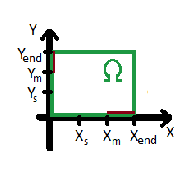
\includegraphics[scale=1.2]{../EllipticEquationSJC/StopCrit.eps}
     \end{center}
	\caption{Stop Criteria Intervals}
	\label{fig:StopCritf}
\end{figure}
There exist start points $x_{s}$ and $y_{s}$ for which the asymptotic conditions
are valid inside the intervals $[x_{s}, x_{end}]$ and $[y_{s}, y_{end}]$. Furthermore, (\ref{asy}) are also valid on intervals $[x_{m}, x_{end}]$ and $[y_{m}, y_{end}]$, where $x_{m}$ and $y_{m}$ are the midpoints i.e.
$x_{m} = (x_{s} + x_{end})/2$ and $y_{m} = (y_{s} + y_{end})/2$. 


At each $k^{th}$ successful iteration $k \in N$, the two expressions in \rf{asy} are approximated by constant functions (zero order polynomial) $c_{x}(x_{i}) = c_{x}$ and $c_{y}(y_{i}) = c_{y}$ with $x_{i} \in [x_{m}, x_{end}]$ and $y_{i} \in [y_{m}, y_{end}]$ respectively.

In between each $k$ iterations, the approximations are evaluated and compared with each other i.e., if the linear fits $c_{x}$ and $c_{y}$
\begin{equation}\label{stopCrit}
|c_{x}^{n} - c_{x}^{(n-k)}| < \epsilon \quad \textrm{and} \quad |c_{y}^{n} - c_{y}^{(n-k)}| < \epsilon
\end{equation}
cease to change significantly between $k$ iterations then the solution has converged. Here the superscript $n$ is the current iteration number and $c_{x}^{n}$ means the value of $c_{x}$ at the n-th iteration.

\subsection{3.4~Basic Algorithm Steps.}
The following are the most important milestones during the implementation of the algorithm.
\\
1) Resolve proper initial condition $(v^0, w^0)$ on the grid $\Omega_h$.  Set parameters $\epsilon$ and $\tau$.
\\
2) Suppose $(v^k, w^k)$ are known. 
\par
2.1) Find current $\theta_k$ from the discrete approximation of \rf{eqtheta};
\par
2.2) Evaluate the solution on the computational boundary;
\par
2.3) Evaluate $\Delta_{h,p}  \widehat{v}^k$ and $\Delta_{h,p}  \widehat{w}^k$;
\par
2.4) Calculate $(\widehat{v}^{k+1}, \widehat{w}^{k+1})$  on the  time level $t^{k+1}$ by the Euler explicit scheme   \rf{eq55};
\par
2.5) Calculate the residual $R^{k+1}_{i,j}$ from \rf{residual} and check the stop condition \rf{stopCrit}.
\par
2.6) Control the time step size $\tau$. Set $t^{k+1}=t^{k}+\tau$.
\\
3) Continue steps 2.1) -- 2.6) with the next time level $t^{k+1}$ till condition (\ref{stopCrit}) is satisfied.

\section{4.~Validation.}\label{validation}

In this section we give several numerical results concerning the verification of  the presented numerical method. 
 We use FDS with different approximation errors and several sets  of  parameters $c$, $\alpha$, $\beta$,  which are shown on each table. 


\begin{center}
\begin{table}[ht]
\centering
		\begin{tabular}{||c|l|ll|ll||}
			\hline
			\hline
      FDS       & $h$ &errors $E_i$in$L_2$&Conv. Rate& errors $E_i$in$L_\infty$&Conv. Rate\\
   			\hline 
					\hline 
      c=0.45    &0.2    &             &            &           &   \\
   $O(h^2)$     &0.1    &~ 0.010413  &            &~0.009363 &   \\
                &0.05   &~ 0.002451  &2.0870  &~0.002258 & 2.0517 \\
               	 \hline 
     c=0.1      &0.2   &             &           &                & \\
     $O(h^2)$   &0.1   &~ 0.009880  &             &~0.008483      &    \\
                &0.05  &~ 0.002332 & 2.0827       &~0.002033      & 2.0609  \\
			\hline
			\hline 	
      c=0.45    &0.2   &            &            &             &    \\
       $O(h^4)$ &0.1   &~ 0.000782   &           &~0.000824  &   \\
                &0.05  &~ 0.000050 & 3.9582    &~0.000054  & 3.9226  \\
					  			\hline 	
     c=0.1      &0.2  &            &               &               &     \\
     $O(h^4)$  &0.1   &~ 0.000678  &              &~0.000662      &        \\
               &0.05  &~ 0.000044 &3.9550        &~0.000044 &  3.9046        \\
			\hline
    \hline
   c=0.45       &0.4   &            &        &                  &      \\
     $O(h^6)$   &0.2   &~ 2.0975e-02 &           &~2.9341e-02      &       \\
     &0.1  &~ 3.5348e-04 &5.8909  &~5.8346e-04 & 5.6521         \\
	  \hline
   c=0.1       &0.4   &             &        &               &        \\
     $O(h^6)$  &0.2   &~ 3.7059e-03  &        &~3.7572e-03     &       \\
   &0.1  &~ 7.4723e-05 &5.6321  &~8.3359e-05&   5.4942       \\
	   \hline
			\hline 
		\end{tabular}
		\caption{Convergence test for  FDS with different approximation errors ($O(h^{2})$, $O(h^{4})$ and $O(h^{6})$). Errors $E_i$ are measured in $L_2$ and $L_\infty$ norms}

\label{tab:a}
\end{table}
\end{center}

 In this series of tests we evaluate the numerical solution of \rf{eq5} using FDS with approximation errors $O(h^2)$, $O(h^4)$, $O(h^6)$ and parameters  
 $\alpha = 1$,   $\beta=3$,  $\epsilon = 10e-5$, 
$L_{x }= 30$, $L_{y} = 30$.
The initial conditions for the artificial parabolic problem \rf{eq55} are taken from  \cite{Ch2011}. 
Using the values of numerical solution on three nested meshes, we compute the numerical rate of convergence (Conv. Rate) in $L_2$ and $L_{\infty}$ mesh norms
by Runge method as $(\log E_1 -\log E_2)/\log 2$.  Here  $v_{[h]}$, $v_{ {[h/2]}  }$ and  $v_{ {[h/4]}  }$ represent the numerical solution over three nested meshes and $E_1=\|v_{[h]}-v_{[h/2]}\|$ , $E_2=\|v_{[h/2]}-v_{[h/4]}\|$.  
Table~\ref{tab:a} contains the errors in $L_2$ and $L_{\infty}$ norms and the corresponding numerical rate of convergence for the numerical solutions obtained by FDS with second, fourth and sixth order of approximation and   velocities  $c=0.1$  or $c=0.45$.
We observe that the experimental rate of convergence approximates well the approximation error of the difference schemes -- the FDS are of  almost the same order of convergence as the order of approximation. An additional observation  is that  for  the same step size $h$ the schemes with higher order of approximation ($O(h^4)$, $O(h^6)$) lead to a more precise solution than the scheme with $O(h^2)$ approximation error. 

\begin{figure}[ht]
	\begin{minipage}[b]{0.5\linewidth}
		\raggedleft
		\includegraphics[width=\linewidth]{../EllipticEquationSJC/solution/SOL2D_bnd25_c090_bt1.eps}
	\end{minipage}
	\begin{minipage}[b]{0.5\linewidth}
		\raggedright
		\includegraphics[width=\linewidth]{../EllipticEquationSJC/solution/SOL2D_bnd25_c050_bt3.eps}
	\end{minipage}
	\begin{minipage}[b]{0.45\linewidth}
		 \raggedleft
		\includegraphics[width=\linewidth]{../EllipticEquationSJC/solution/SOL3D_bnd25_c090_bt1.eps}
		\centerline{$c = 0.9$, $\beta = 1$}
	\end{minipage}
	\begin{minipage}[b]{0.5\linewidth}
		 \raggedright
		\includegraphics[width=\linewidth]{../EllipticEquationSJC/solution/SOL3D_bnd25_c050_bt3.eps}
		\centerline{$c = 0.5$, $\beta = 3$}
	\end{minipage}
	\caption{2D and 3D profiles of the numerical solution $u$ to \rf{eqtheta} and \rf{eq5}}
	\label{fig:solutions}
\end{figure}

\section{5.~Results.}\label{results}

In this section we apply the presented  numerical method  to study the characteristic properties of the obtained numerical solution.  Many parametric dependencies of the numerical solution,  discovered in \cite{Ch2012,Ch2011}, such as dependence of the solution's shape on the velocity $c$ and on the relative dispersion parameter $\beta$, are confirmed here once again.
 We   also compare  the best--fit  formulae,  built up in \cite{Ch2011}, with the numerical solution  developed here. Such comparison is still missing in the literature.
Recall that the best--fit formulae   are used as initial data for our algorithm. 

\subsection{5.1~Solution residual.}

\begin{figure}[htbp]
	\begin{minipage}[b]{0.5\linewidth}
		 \centering
		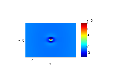
\includegraphics[width=\linewidth]{../EllipticEquationSJC/residual/residual_bt5c03.eps}
		\centerline{$\beta = 5$, $c = 0.3$}
	\end{minipage}	
	\begin{minipage}[b]{0.5\linewidth}
		\centering
		 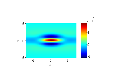
\includegraphics[width=\linewidth]{../EllipticEquationSJC/residual/residual_bt1c09.eps}
	\centerline{$\beta = 1$, $c = 0.9$ }
	\end{minipage}
		\caption{Residual at the last step of iteration process \rf{eq55} }
		\label{resid}
\end{figure}

On the left picture in Figure~\ref{resid} we present  the residual \rf{residual}, saved on the last time level of the numerical scheme \rf{eq55},  for $\beta = 5$ and $c = 0.3$, while the residual, evaluated for problem with $\beta = 1$, $c = 0.9$, is demonstrated on the right part of Figure~\ref{resid}. Here  $\epsilon =10e-6$ and the FDS is of 6th order of approximation. In these cases the difference between the last two iterations is $3.7749e-007$ for the first data set and $1.2726e-007$ for the second data set. These results show that the  equation \rf{eq3} is satisfied numerically with high accuracy. 
Note that similar results about the residual for the numerical scheme in \cite{Ch2012} are not reported there. Concerning the best--fit formulae from \cite{Ch2011} -- it is obvious to conclude from these formulae that the third, fourth and so on derivatives of the best--fit solution are unbounded in the neighborhood of the point $(0,0)$. Thus  
the residual, which includes fourth order derivatives of the solution, could not be considered and evaluated in the classical sense. Therefore the equation \rf{eq3} is not satisfied in the neighborhood of the origin by the best--fit formulae  from \cite{Ch2011}!
 \begin{center}
\begin{table}[ht]
\centering
		\begin{tabular}{||c|l|ll|ll||}
			\hline
			\hline
      FDS       & $h$ &errors in $L_2$&Conv. Rate& errors in $L_\infty$&Conv. Rate\\
   			\hline 
					\hline 
      c=0.45    &0.8    &             &            &           &   \\
   $O(h^2)$     &0.4    &~ 2.9698e-01  &            &~4.2497e-01 &   \\
                &0.2   &~ 6.8742e-02  &~~2.1111  &~8.6465e-02 &~~2.2972 \\
               	 \hline 
     c=0.1      &0.8   &             &           &                & \\
     $O(h^2)$   &0.4   &~ 3.4849e-01  &             &~3.0271e-01      &    \\
                &0.2  &~ 8.7696ee-02 &~~1.9905       &~7.5691e-02      &~~1.9998  \\
			\hline
			\hline 	
      c=0.45    &0.8   &            &            &             &    \\
       $O(h^6)$ &0.4   &~ 1.0766e+00   &           &~1.2316e+00  &   \\
                &0.2  &~ 3.5768e-02 &~~4.91117    &~5.8927e-02  &~~4.3855  \\
					  			\hline 	
     c=0.1      &0.8  &            &               &               &     \\
     $O(h^6)$  &0.4   &~ 8.0095e-01  &              &~9.8911e-01      &        \\
               &0.2  &~ 1.5680e-02&~~5.6747        &~2.1238e-02 &~~5.5414       \\
		   \hline
			\hline 
		\end{tabular}
		\caption{Errors  in $L_2$ and $L_\infty$ norms and  convergence  rate for  fourth order discrete derivative  evaluated by FDS with $O(h^2)$ and $O(h^6)$ approximation errors}
\label{tab:fourth-der}
\end{table}
\end{center}

\subsection{5.2~Solution derivatives.}

We have mentioned already that the best--fit formulae from \cite{Ch2011} have singularities near the origin. 
Now we demonstrate  that the discrete fourth order derivatives of the numerical solution converge numerically as the step size $h$ goes to zero.
We apply the Runge test, evaluating the discrete fourth order derivative $v_{\widehat{xxxx}}$ of the solution on three nested meshes with step sizes $h$, $h/2$, $h/4$ (see Section~\rf{validation}).  The results are demonstrated on Table~\ref{tab:fourth-der}.  
We conclude that the discrete  derivative $v_{\widehat{xxxx}}$ is bounded and converges numerically for $h\rightarrow 0$. The tests for the other fourth order derivatives are similar to the derivative $v_{xxxx}$ and we do not present them here.

\subsection{5.3~Solution shape.}

\begin{figure}[ht]
	\begin{minipage}[b]{0.5\linewidth}
		\raggedleft
		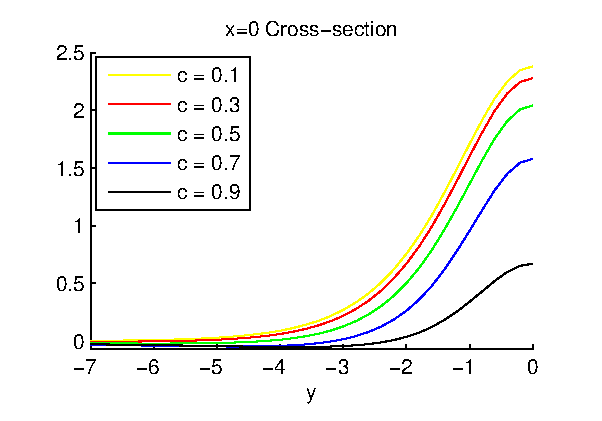
\includegraphics[width=\linewidth]{../EllipticEquationSJC/cross-sections/c=01__09beta=1x=0.eps}
	\end{minipage}	
	\begin{minipage}[b]{0.5\linewidth}
		\raggedright
		 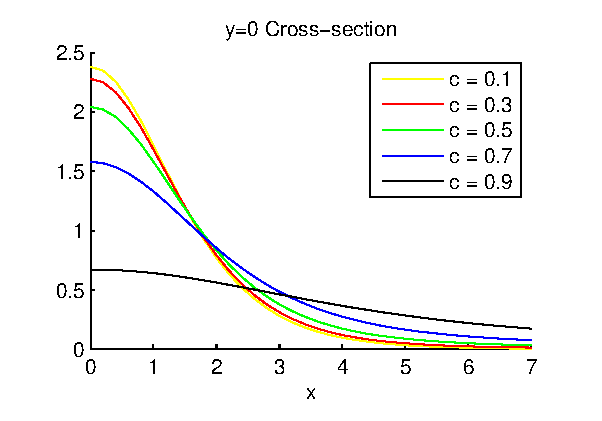
\includegraphics[width=\linewidth]{../EllipticEquationSJC/cross-sections/c=01__09beta=1y=0.eps}
	\end{minipage}
	\begin{minipage}[b]{0.5\linewidth}
		\raggedleft
		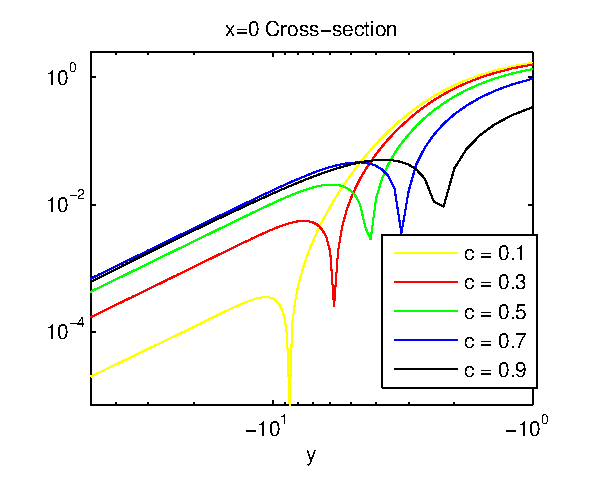
\includegraphics[width=\linewidth]{../EllipticEquationSJC/cross-sections/c=01__09beta=1Logx=0.eps}
	\end{minipage}	
	\begin{minipage}[b]{0.5\linewidth}
		\raggedright
		 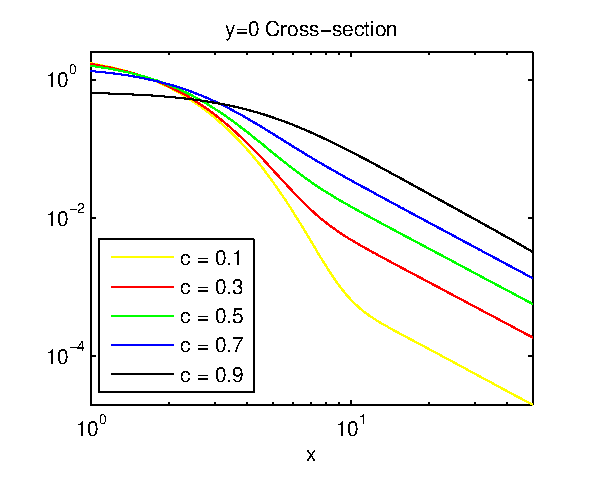
\includegraphics[width=\linewidth]{../EllipticEquationSJC/cross-sections/c=01__09beta=1Logy=0.eps}
	\end{minipage}
	\caption{Cross--sections of the numerical solution for $\beta=1$ and several  $c$}
	\label{profilesSpeedVarying}
\end{figure}

\begin{figure}[htbp]
	\begin{minipage}[b]{0.48\linewidth}
		\raggedleft
		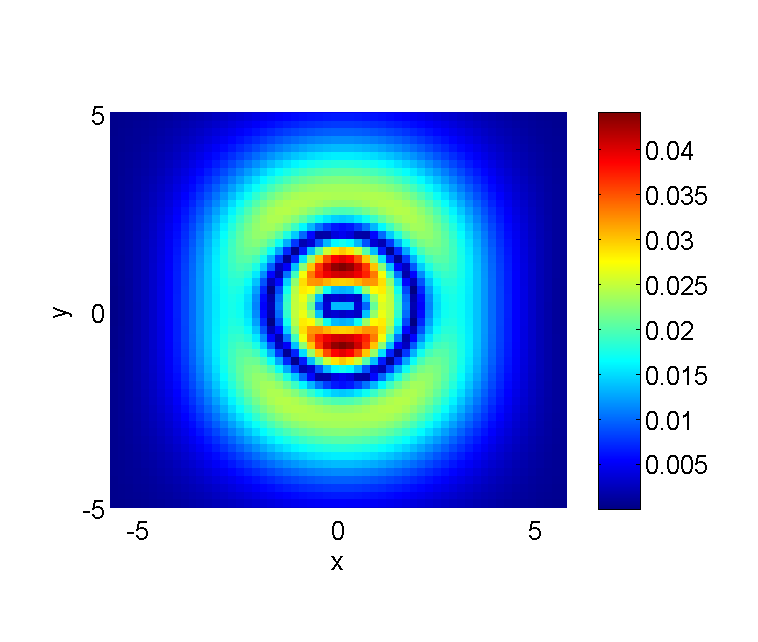
\includegraphics[width=\linewidth]{../EllipticEquationSJC/differences/difference_c=03_beta=1.eps}
	\end{minipage}
	\begin{minipage}[b]{0.48\linewidth}
		 \raggedright
		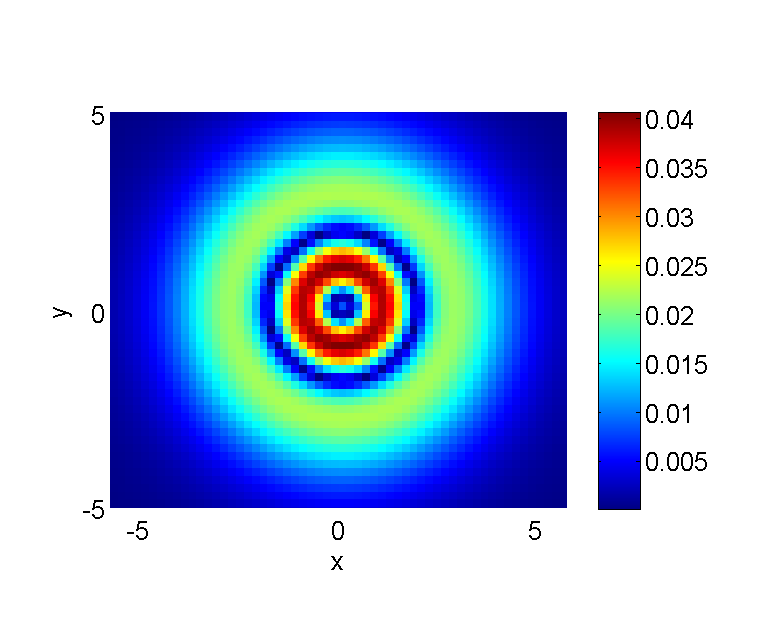
\includegraphics[width=\linewidth]{../EllipticEquationSJC/differences/difference_c=01_beta=1.eps}
	\end{minipage}
	\begin{minipage}[b]{0.48\linewidth}
		\raggedleft
		 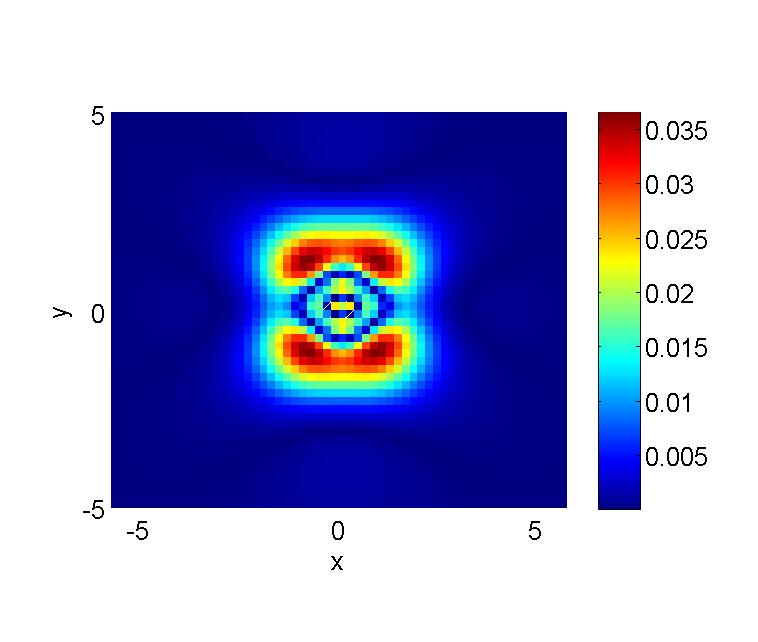
\includegraphics[width=\linewidth]{../EllipticEquationSJC/differences/difference_c=03_beta=3.eps}
	\end{minipage}
	\begin{minipage}[b]{0.48\linewidth}
		\raggedright
		 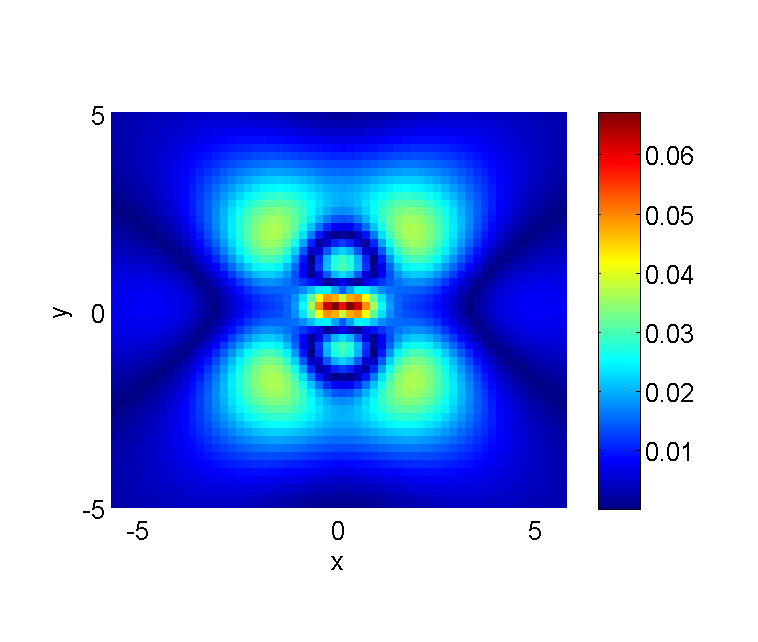
\includegraphics[width=\linewidth]{../EllipticEquationSJC/differences/difference_c=05_beta=1.eps}
	\end{minipage}
	\begin{minipage}[b]{0.48\linewidth}
		\raggedleft
		 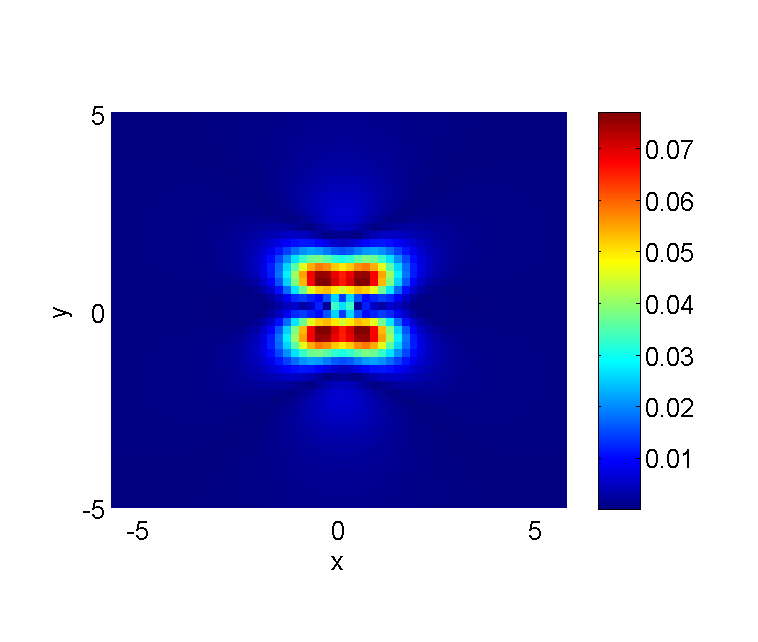
\includegraphics[width=\linewidth]{../EllipticEquationSJC/differences/difference_c=03_beta=5.eps}
		\centerline{$c=0.3$}
		\centerline{$\beta = 1,3,5$ (top to bottom) }
	\end{minipage}
	\begin{minipage}[b]{0.48\linewidth}
		\raggedright
		 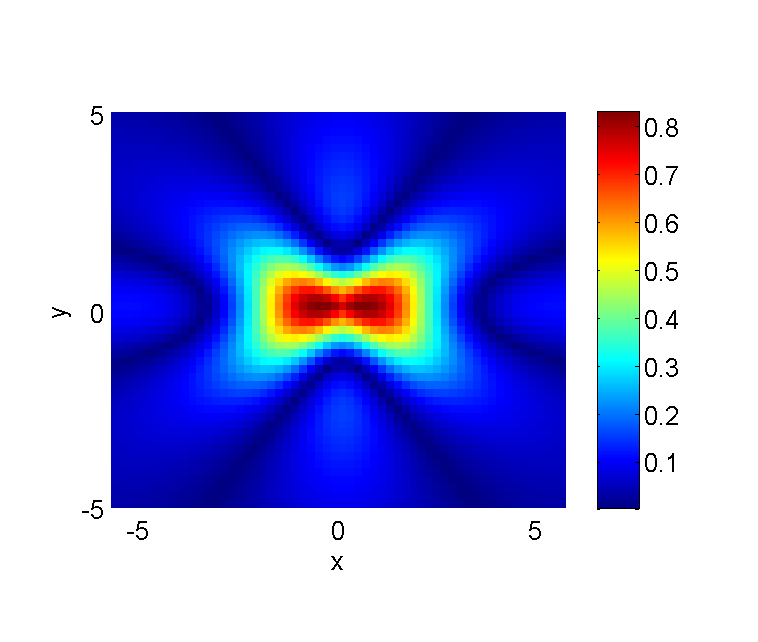
\includegraphics[width=\linewidth]{../EllipticEquationSJC/differences/difference_c=09_beta=1.eps}
		\centerline{$\beta = 1$}
		\centerline{$c = 0.1, 0.5, 0.9$ (top to bottom)}
	\end{minipage}
	\caption{Difference between the numerical solution $v$ and best fit formulae $v^*$ from \cite{Ch2011} }
	\label{fig:difference}
\end{figure}

First, two aspects of the solution for different combinations of  $c$ and $\beta$   are plotted  on Figure~\ref{fig:solutions}. Both numerical solutions are computed on the  domain $\Omega = [0, 25]\times [0, 25]$ with $h = 0.1$ and then extended symmetrically to $ [-25, 25]\times [-25, 25]$. 
Only the essential part of the wave (near the center) is shown on these pictures. Top figures are level plots showing the waves from above and the bottom figures are 
three dimensional showing the structure of the wave in space. 



We perform a detailed study   of the numerical solution's shape with respect to main parameters -- the relative dispersion $\beta=\beta_1 / \beta_2$ and the velocity $c$.
 Figure~\ref{profilesSpeedVarying} shows different aspects of the solution at $x=0$ and $y=0$ cross--sections. The parameter $\alpha$  is fixed as one ($\alpha = 1$) but  parameters $\beta $ and $c$ vary. We apply  the computational procedure with  $L_x = L_y = 50$, $h = 0.2$, $\epsilon = 1.0e-06$. 
On Figure~\ref{profilesSpeedVarying}, parameter $\beta=1$ is held constant and the wave dependence on the phase velocity  $c$ for $c=0.1, 0.3, 0.5, 0.7, 0.9$ is demonstrated.  Linear plots of the solution are presented on the upper row while  log--log plots of the absolute value of the solution are shown on the lower part.  These types of plots help us to establish the size of the computational box. 

One can observe that as the phase velocity $c$ increases the wave's support  along $x$ direction increases too, but the maximum of the wave decreases. The linear part of the solution on the log--log plots is under the governance of the boundary function.

\bigskip


\section{6.~Comparison with best--fit formulae from \cite{Ch2011}.}

\begin{center}
\begin{table}[ht]
\centering
\resizebox{12cm}{!} {
		\begin{tabular}{|l|c|l l| c|l|c|l l|}
			\cline{1-4}\cline{6-9}
$\beta$&c&$\|v^*-v \|_{\infty }$&$\|v^*-v \|_{2 }$& &$\beta$& c&$\|v^*-v \|_{\infty }$&$\|v^*-v \|_{2 }$\\
			\cline{1-4}\cline{6-9}
1&     &4.4002e-02 & 1.4371e-01 & &    1& 0.1& 4.0554e-02  &1.4802e-01\\
3& 0.3 &3.6519e-02 & 9.0714e-02& &    1& 0.5& 6.7063e-02  &1.6766e-01\\
5&     &7.6927e-02 & 1.2936e-01 & &    1& 0.9&  8.2821e-01 &2.1671e0\\
			\cline{1-4}\cline{6-9}
\end{tabular}
}
		\caption{Differences between the numerical solution $v$ and best--fit solution $v^*$ from \cite{Ch2011}.}
\label{tab:first-der-t}
\end{table}
\end{center}

Figure~\ref{fig:difference} and Table~\ref{tab:first-der-t} demonstrate the  absolute value of the difference between  the solution $v^*$ by formulae \cite{Ch2011}  and the final solution of our procedure.

On the left side of Figure~\ref{fig:difference} the phase velocity $c = 0.3$ is fixed  and $\beta$ changes. On the right side  the dispersion parameter $\beta=1$ is kept constant while $c$ changes. The experiments are done on a $[-50,  50] \times [-50,50]$  domain  but only the results near the zero point are plotted. For each of the examples shown on Figure~\ref{fig:difference} more detailed estimate (using numbers) is given in Table~\ref{tab:first-der-t}. The difference is measured in the maximal and $L_2$ norms. One observes that for larger wave velocities $c$ and dispersion parameters $\beta$ the distinction becomes more pronounced. For example, for $\beta =1$ and $c=0.9$ the difference between the numerical solution obtained in this paper and the formulae  $v^*$ from \cite{Ch2011} becomes $\approx 0.8$ !


\bigskip

\section{7.~Conclusion.}
Fourth and sixth order finite difference schemes are applied for numerical evaluation of the stationary traveling wave solutions to the Boussinesq equation in this paper. The high accuracy of the method applied is demonstrated on several experiments. The numerical solution obtained here performs similarly to the numerical solutions given in \cite{Ch2012,Ch2011} with respect to solution shape and the dependence on the velocity $c$ and relative dispersion $\beta$. 
The best--fit approximation formulae from  \cite{Ch2011} fail to satisfy the initial equation in the classical sense in the neighborhood of the origin. 
In the future, we will exploit the obtained stationary traveling wave solutions as initial data to the corresponding Boussinesq equation in order to seek two dimensional solitary wave solutions to \rf{eq1}.

\bigskip

\fi


\section{Увод}
Парадигматично уравнение на Бузинеск
\be\label{problemCh}
...
\ee


\section{Смяна на променливите}

За удобство правим следната смяна на променливите (виж \cite{ref25}):

\begin{align}
x = \sqrt{\beta_1} \bar{x}, \quad y = \sqrt{\beta_1} \bar{y}, \quad t = \sqrt{\beta_1} \bar{t} \nonumber
\end{align}
която променя основното уравнение \rf{problemCh} в
\be\label{problemVC}
 \beta (I-\Delta) \frac{\partial^2}{\partial t^2}u= 
(I-\Delta)\Delta u +\Delta( (\beta - 1 )u - \alpha \beta u^2 )
\ee
където $\beta = \beta_1/\beta_2$. 

\section{Дискретизация}
Неограничената област на уравнението е заменена с достатъчно голям правоъгълник $\Omega$, така че стойностите на неизвестната функция $u$ са достатъчно малки близо до границата $\partial \Omega$. Използвана е равномерна мрежа  $\Omega_h$ дефинирана по следния начин:

\begin{align}\label{Omega}
\Omega_h = \{(x_i,y_j): x_i = (i-\frac{N_x-1}{2})h, \; &y_j = (j-\frac{N_y-1}{2})h, \nonumber\\
                                         & i = 0,\cdots, N_x, j = 0 ,\cdots , N_y \},
\end{align}
където $N_x$ и $N_y$ описват броя на точките по осите $x$ и $y$, а стъпката по пространството $h$ удовлетворява $h =2 L_x/(N_x-1) =2 L_y/(N_y-1)$.
С $2 L_x$ и $2 L_y$ са означени размерите на $\Omega_h$ по осите $x$ и $y$. Дискретния времеви интервал е дефиниран аналогично чрез
$$
T_{\tau} = \{(t_k): t_k = k\tau, k = 0,\cdots ,N_t \},
$$
където с $\tau = T/N_t$ сме означили стъпката по времето. Стойността на неизвестната функция $u$ в точка от мрежата $(x_i,y_j,t_k)$ е означена с $u_{i,j}^{(k)}$,т.е. долния индекс се използва за пространствената дискретизация, а горния за времева дискретизация. Така може да се дефинира и следната редица от матрици $\left(V^{(k)}\right)^T := (u_{i,j}^{(k)})$ при $k=0,..,N_t$, които ще спомогнат за представянето на изчислителните сметки при оператора на Лаплас $\Delta_h$. За неговата дискретизация са използвани централни крайни разлики с различна степен на апроксимация:
\begin{equation}\label{fdx}
u_{\widehat{xx},p}(x,y) :=  \frac{1}{h^2} \sum\limits_{i=-p/2}^{p/2} d_i u(x+ih, y_j).
\end{equation}
като теглата $d_i$ са взети от \cite{forn} и са описани в Таблица \ref{table:A00}. Производните по $y$ се дефинират аналогично със същия шаблон:
\begin{equation}\label{fdy}
u_{\widehat{yy},p}(x,y) :=  \frac{1}{h^2} \sum\limits_{i=-p/2}^{p/2} d_i u(x, y_j+ih).
\end{equation}

\begin{table}[ht]
\centering
\small
		\begin{tabular}{||c|l|l|l|l|l|l|l||}
			\hline
			\hline
            $p=2$          &          &                                 &     1      &   -2   &    1    &    &        \\
   			\hline 
			\hline 
           $p=4$          &                            &   $-\frac{1}{12}$     &     $\frac{4}{3}$      &   $-\frac{5}{2} $     &    $\frac{4}{3}$    &  $-\frac{1}{12}$   &        \\
	   \hline
			\hline 
            $p=6$        &   $\frac{1}{90}$       &     $-\frac{3}{20}$     &    $\frac{3}{2}$      &    $-\frac{49}{18}$   &    $\frac{3}{2}$    & $-\frac{3}{20}$    &    $\frac{1}{90}$       \\
	   \hline
			\hline 
		\end{tabular}
	\caption{Централни крайни разлики използвани при апроксимацията на оператора на Лаплас.}
	\label{table:A00}
\end{table}
Грешката от дискретните апроксимации \rf{fdx}, \rf{fdy} е $O(h^p)$ в зависимост от избора на $p$. Използвайки мрежата $\Omega_h$ и Таблица \ref{table:A00} при $p=2$ може да се дефинират следните диференчни оператори:
\begin{align}
u_{\bar{x}x}(x_i,y_j) = u_{\widehat{xx},2}(x_i,y_j) = \frac{1}{h^2}(u_{i+1,j} - 2u_{i,j} + u_{i-1,j}), i = 1,.., N_x-1, j = 0,.., N_y \nonumber\\
u_{\bar{y}y}(x_i,y_j) = u_{\widehat{yy},2}(x_i,y_j) = \frac{1}{h^2}(u_{i,j+1} - 2u_{i,j} + u_{i,j-1}), i = 0,.., N_x, j = 1,.., N_y-1 \nonumber
\end{align}
Използвайки времевата област $T_{\tau}$ се дефинират диференчните оператори:
\begin{align}
& u^{(k)}_{\bar{t}t}(x_i,y_j,t_k) = \frac{1}{\tau^2}(u_{i,j}^{(k+1)} - 2u_{i,j}^{(k)} + u_{i,j}^{(k-1)}), k = 1,..,N_t-1 \nonumber\\
& u^{(k)}_{t}(x_i,y_j,t_k) =  \frac{1}{\tau}(u_{i,j}^{(k+1)} - u_{i,j}^{(k)}), k = 0,.., N_{t}-1 \nonumber\\
& u^{(k)}_{\bar{t}}(x_i,y_j,t_k) =  \frac{1}{\tau}(u_{i,j}^{(k)} - u_{i,j}^{(k-1)}), k = 1,.., N_{t} \nonumber.
\end{align}
Дискретния оператор на Лаплас в произволна точка от вътрешността на мрежата $(x_i, y_j) \in \Omega_h \setminus \partial\Omega$ се изразява с 
$$\Delta_{h,2}u(x_i, y_j, t_k) :=  u_{\bar{x}x}(x_i, y_j, t_k) + u_{\bar{y}y}(x_i, y_j, t_k),$$
а при произволно $p$ важи следната дефиниция:
\be\label{deltaHSingle}
\Delta_{h,p} u(x_i, y_j, t_k) :=  u_{\widehat{xx},p}(x_i, y_j, t_k) + u_{\widehat{yy},p}(x_i, y_j, t_k).
\ee
Последното уравнение може да се запише в матричен вид отчитайки всички вътрешни точки от мрежата:
\be\label{DeltaH}
\left( \Delta_{h,p}(N_x-2)*(V^{(k)})^T\right)^T + \Delta_{h,p}(N_y-2)*V^{(k)} := \Delta_{h,p} (V^{(k)}) ,
\ee
където $\Delta_{h,p}(N_x-2) \in \RR^{(N_x-2) \times (N_x-2)}$ и $\Delta_{h,p}(N_y-2) \in \RR^{(N_y-2) \times (N_y-2)}$ са квадратни лентови матриции с една и съща структура, но с различна големина, a $(.)^T$ е транспонирата матрица. При $p=2$ и произволно естествено число $n>2$ 
\[
\Delta_{h,2}(n) = \frac{1}{h^2}
\begin{bmatrix}
    \dots       & \dots        &     \dots   &   \dots        & 0   \\
    1               & -2            &   1           &   0               & \vdots    \\
        0           & \ddots        &    \ddots    &   \ddots       &  0 \\ 
    \vdots       &     0            &  1     	& -2    	   & 1 \\
    0               & \dots          &  \dots         & \dots  	   & \dots \\
\end{bmatrix}
\]
При $p=4$ и произволно естествено число $n>4$ 
\[
\Delta_{h,4}(n) = \frac{1}{h^2}
\begin{bmatrix}
    \dots		& \dots            	& \dots		&   		 \dots  &    \dots      	   &   0           & 0    \\
    \dots    	           &\dots            	& \dots		&   		\dots   &   \dots      	   	   &   0	           & \vdots  \\
    -\frac{1}{12}	& \frac{4}{3}         	& -\frac{5}{2}	&  \frac{4}{3}    	 &   -\frac{1}{12}	  &      0           &\vdots    \\
        0           		& \ddots        	&    \ddots   		 &   \ddots      	 &     \ddots      	  &  \ddots        &    0 \\	
\\
   \vdots      		 & 0           		 &  -\frac{1}{12}	& \frac{4}{3}    	& -\frac{5}{2}	&  \frac{4}{3}  &   -\frac{1}{12} \\
    \vdots    		 & 0        		 &	 \dots     	&  \dots              	&\dots 		 &  \dots 	&\dots   	\\
    0              		 & 0        		 &	 \dots     	&  \dots             	 &\dots 		 &  \dots 	&\dots 	\\
\end{bmatrix}
\]
При $p=6$ и произволно естествено число $n>6$ е показана само структурата на лентата  (виж Таблица \ref{table:A00}):
\[
\begin{bmatrix}
    \frac{1}{90}	& -\frac{3}{20}	& \frac{3}{2}         	& -\frac{49}{18}	&  \frac{3}{2}    	 &   -\frac{3}{20}	  &      \frac{1}{90}
\end{bmatrix}
\]
като тук първите три и последни три реда от матрицата са все още предмет на дефиниране, т.е. в хоризонталните многоточия на горепосочените матрици $\Delta_{h,p}(n)$ трябва да се дефинира граничното условие заложено в ПУБ по подходящ начин.

\section{Нулево гранично условие}

Пространството от функции, за които е изпълнено $f_b(x) = 0$ и $\Delta f_b(x) = 0$ по границата $\partial\Omega$ се дефинира чрез
\be\label{funSpace}
J:=\{ f_b : \Omega \rightarrow R | f_b(x) = 0, \Delta f_b(x) = 0, x \in \partial\Omega\}
\ee
Това пространство е в съответстие на граничните условия зададени в ПУБ. Дискретните оператори $\Delta_{h,p}(N_x-2) \in \RR^{(N_x-2) \times (N_x-2)}$ и $\Delta_{h,p}(N_y-2) \in \RR^{(N_y-2)\times(N_y-2)}$  използват централни крайни разлики с 3, 5 и 7 точки съответно при различните апроксимации $O(h^2)$, $O(h^4)$ и $O(h^6)$ на вторите производни. По и близо до границата се прилагат други шаблони възползвайки се от свойствата на функционалното пространство. При $p=2$ имаме, че 
\[
\Delta_{h,2}(N_x-2) = \frac{1}{h^2}
\begin{bmatrix}
    -2	       & 1        &     \dots   &   \dots        & 0   \\
    1               & -2            &   1           &   0               & \vdots    \\
        0           & \ddots        &    \ddots    &   \ddots       &  0 \\ 
    \vdots       &     0            &  1     	& -2    	   & 1 \\
    0               & \dots          &  \dots         & 1  	   & -2 \\
\end{bmatrix},
\]
защото $u \in J$ и $u(x_0, y_j, t_k) = u(x_{N_x}, y_j, t_k) = 0$. По същия начин, но с различна големина, изглежда и матрицата $\Delta_{h}(N_y-2)$, защото $u \in J$ и $u(x_i, y_0, t_k) = u(x_i, y_{N_y}, t_k) = 0$.  При $p=4$ имаме, че 
\[
\Delta_{h,4}(N_x-2) = \frac{1}{h^2}
\begin{bmatrix}
     -\frac{38}{15}	& \frac{29}{20}       & -\frac{2}{15}	&    \frac{1}{120}     &    \dots      	   &   0           & 0    \\
    \frac{4}{3}          &-\frac{5}{2}    	& \frac{4}{3}	&   -\frac{1}{12}	  &   \dots      	  &   0	           & \vdots  \\
    -\frac{1}{12}	& \frac{4}{3}         	& -\frac{5}{2}	&  \frac{4}{3}    	 &   -\frac{1}{12}	  &      0           &\vdots    \\
        0           		& \ddots        	&    \ddots   		 &   \ddots      	 &     \ddots      	  &  \ddots        &    0 \\	
\\
   \vdots      		 & 0           		 &  -\frac{1}{12}	& \frac{4}{3}    	& -\frac{5}{2}	&  \frac{4}{3}   &   -\frac{1}{12} \\
    0      		 &  \dots           	 &   0     		& -\frac{1}{12} 	 & \frac{4}{3} 	 & -\frac{5}{2}  &  \frac{4}{3}\\
    0              		 & \dots          	&  0              		 &\frac{1}{120} 	 &  -\frac{2}{15} 	& \frac{29}{20} & -\frac{38}{15}\\
\end{bmatrix}
\]
Вторият и предпоследният редове на матрицата $\Delta_{h,4}(N_x-2)$ се обясняват с условието, че $u \in J$ и съответно $u(x_0, y_j, t_k) = u(x_{N_x}, y_j, t_k) = 0$ както е при $O(h^2)$ апроксимацията. 

\begin{figure}%{r}{50mm}
     \begin{center}
     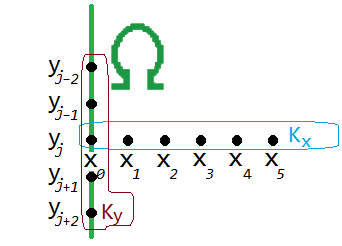
\includegraphics[scale=.5]{LeftBoundary.png}
     \end{center}
	\caption{Шаблон с $O(h^4)$ апроксимация при имплементация на $\Delta_h$ оператора по лявата граница на областта.}
	\label{fig:LeftBoundary}
\end{figure}

Условието $\Delta u(x_0, y, t) = 0$ върху лявата граница на областта се описва с крайна разлика напред $K_x[0,1,2,3,4,5]$ за втората производна по $x$ и централна крайна разлика $K_y[-2,-1,0,1,2]$ за втората производна по $y$ (виж Фигура \rf{fig:LeftBoundary}). С вектора в квадратните скоби на крайните разлики $K_x$ и $K_y$ се обозначава релативната позиция на използваните възли. Резултатът от произвнодните пресметнати посредством $K_x$ и $K_y$ се отнася за възела обозначен с нула. Понеже $u(x_0, y, t) = 0$ следва, че събираемите от $K_y[-2,-1,0,1,2]$ заедно с първия елемент от $K_x[0,1,2,3,4,5]$ са нула. Като последното важи за всяка крайна разлика $K_y$ с точки върху границата $\partial \Omega$. Ако означим с $\bar c_0, \bar c_1, .., \bar c_5$ теглата на крайната разлика напред $K_x[0,1,2,3,4,5]$ и с $\bar d_0, \bar d_1,.., \bar d_5$ теглата на крайната разлика $K_x[-1,0,1,2,3,4]$ се получава че:
\begin{align}
\sum\limits_{i=0}^{5} \bar c_i u(x+ih, y_j) = \sum\limits_{i=1}^{5} \bar c_i u(x+ih, y_j) = 0 &  \quad | \frac{\bar d_5}{\bar c_5} \nonumber\\
\bar d_5 u(x+5h, y_j) = -\sum\limits_{i=1}^{4} \bar c_i u(x+ih, y_j) & \nonumber
\end{align}
Последният член $u(x+5h, y_j)$ от $K_x[0,1,2,3,4,5]$ е изразен чрез останалите и може да се замести в $K_x[-1,0,1,2,3,4]$ както следва:
\begin{align}\label{fdResult}
&\sum\limits_{i=0}^{5} \bar d_i u(x+ih, y_j) = \sum\limits_{i=1}^{5} \bar d_i u(x+ih, y_j)  =  \\
&= \sum\limits_{i=1}^{4} \bar d_i u(x+ih, y_j) -\sum\limits_{i=1}^{4} \bar c_i u(x+ih, y_j) = \sum\limits_{i=1}^{4} \left( \bar d_i - \frac{\bar d_5}{\bar c_5} \bar c_i \right) u(x+ih, y_j) \nonumber
\end{align}
Понеже $K_x[0,1,2,3,4,5]$ и $K_x[-1,0,1,2,3,4]$ са крайни разлики апроксимиращи втора производна с грешка $O(h^4)$ (\cite{forn}) то полученият резултат \rf{fdResult} е със същата грешка $O(h^4)$. Теглата $\bar c_i$ и $\bar d_i$ при $p=4$ са дефинирани както следва (\cite{forn}):
\begin{align}
&\bar c_i, i = 0,..,5 \iff \frac{15}{4}, -\frac{77}{6}, \frac{107}{6}, -13, \frac{61}{12}, -\frac{5}{6} \\
&\bar d_i, i = 0,..,5 \iff \frac{5}{6}, -\frac{5}{4}, -\frac{1}{3}, \frac{7}{6}, -\frac{1}{2}, \frac{1}{12} 
\end{align}
и след като се заместят в \rf{fdResult} се получават коефициентите от първия ред на матрицата $\Delta_{h,4}(N_x-2)$. При последния ред се прилагат аналогични разсъждения върху дясната граница на областта, но вече се използва крайна разлика назад $K_x[-4,-3,-2,-1,0]$ за втората производна по $x$ при пресмятането на дискретния Лапласиан. 

Аналогични разсъждения се прилагат за горната и долната граници на областта при другата матрица $\Delta_{h,4}(N_y-2)$, която се използва за изчисляването на втората производна по $y$ и затова нейната структура е същата.

При $p=6$ матрицата $\Delta_{h,6}(N_x-2)$ има следния вид:
\[
\frac{1}{h^2}
\begin{bmatrix}
   -\frac{327}{140}	& \frac{191}{168}	&   \frac{167}{1134}	& -\frac{1}{7}    		 & \frac{19}{420}	& -\frac{77}{13331}   &    0      	   	&   \dots           & 0    \\
    \frac{54}{35}    	&-\frac{235}{84}   	&    \frac{884}{567}    &-\frac{5}{28}  	 	& \frac{2}{105}		&  -\frac{11}{11340}	 &   0      	   	&   \dots	       & \vdots  \\
    -\frac{3}{20}		& \frac{3}{2}         	& -\frac{49}{18} 	&  \frac{3}{2}		&  -\frac{3}{20}    	 &   \frac{1}{90}    	 &  0			&     \dots         &\vdots    \\
    \frac{1}{90}		& -\frac{3}{20}		& \frac{3}{2}         	& -\frac{49}{18} 	&  \frac{3}{2}		&  -\frac{3}{20}    	 &   \frac{1}{90} &     \dots         &\vdots    \\
        0           		& \ddots        		&         \ddots           	& \ddots        		&    \ddots   		&   \ddots      		 &     \ddots    	&  \ddots          &    0 \\	
\\
   \vdots      		&            		 	&    	0	      		& \frac{1}{90}		& -\frac{3}{20}		& \frac{3}{2}         	& -\frac{49}{18}	&  \frac{3}{2}  &  -\frac{3}{20} \\
    0      			&              	 	&    0      		&   -\frac{11}{11340}	 	&    \frac{2}{105} 	&  -\frac{5}{28} 	& \frac{884}{567} &-\frac{235}{84} &  \frac{54}{35}\\
    0              	& 	          		&    0              	&  -\frac{77}{13331}    		&  \frac{19}{420}&-\frac{1}{7}	 &  \frac{167}{1134} 	& \frac{191}{168}  &  -\frac{327}{140}\\
\end{bmatrix}
\]
Третият и предпредпоследният ред на матрицата $\Delta_{h,6}(N_x-2)$ се обясняват с условието, че $u \in J$ и съответно $u(x_0, y_j, t_k) = u(x_{N_x}, y_j, t_k) = 0$ както е при $O(h^2)$ апроксимацията. 


Условието $\Delta u(x_0, y, t) = 0$ върху лявата граница на областта се описва с крайна разлика напред $K_x[0,1,2,3,4,5,6,7]$ за втората производна по $x$ и централна крайна разлика $K_y[-3,-2,-1,0,1,2,3]$ за втората производна по $y$ както е направено при $p=4$ (виж Фигура \rf{fig:LeftBoundary}), но с разликата че тук по-високият порядък на апроксимация изисква два възела в повече. Понеже $u(x_0, y, t) = 0$ следва, че събираемите от $K_y[-3,-2,-1,0,1,2,3]$ заедно с първия елемент от $K_x[0,1,2,3,4,5,6,7]$ са нула. Като последното важи за всяка крайна разлика $K_y$ с точки върху границата $\partial \Omega$. Ако означим с $\bar c_0, \bar c_1, .., \bar c_7$ теглата на крайната разлика напред $K_x[0,1,2,3,4,5,6,7]$ и с $\bar d_0, \bar d_1,.., \bar d_7$ теглата на крайната разлика $K_x[-1,0,1,2,3,4,5,6]$ се получава че:
\begin{align}\label{deltaOh6Zero}
\sum\limits_{i=0}^{7} \bar c_i u(x+ih, y_j) = \sum\limits_{i=1}^{7} \bar c_i u(x+ih, y_j) = 0 &  \quad | \frac{\bar d_7}{\bar c_7} \nonumber\\
\bar d_7 u(x+7h, y_j) = -\sum\limits_{i=1}^{6} \bar c_i u(x+ih, y_j) & 
\end{align}
Последният член $u(x+7h, y_j)$ от $K_x[0,1,2,3,4,5,6,7]$ е изразен чрез останалите и може да се замести в $K_x[-1,0,1,2,3,4,6]$ както следва:
\begin{align}\label{fdResultOh6}
&\sum\limits_{i=0}^{7} \bar d_i u(x+ih, y_j) = \sum\limits_{i=1}^{7} \bar d_i u(x+ih, y_j)  =  \\
&= \sum\limits_{i=1}^{6} \bar d_i u(x+ih, y_j) -\sum\limits_{i=1}^{6} \bar c_i u(x+ih, y_j) = \sum\limits_{i=1}^{6} \left( \bar d_i - \frac{\bar d_7}{\bar c_7} \bar c_i \right) u(x+ih, y_j) \nonumber
\end{align}
Понеже $K_x[0,1,2,3,4,5,6,7]$ и $K_x[-1,0,1,2,3,4,5,6]$ са крайни разлики апроксимиращи втора производна с грешка $O(h^6)$ (\cite{forn}) то полученият резултат \rf{fdResultOh6} е със същата грешка $O(h^6)$. Теглата $\bar c_i$ и $\bar d_i$ при $p=6$ са дефинирани както следва (\cite{forn}):
\begin{align}
&\bar c_i, i = 0,..,7 \iff \frac{469}{90}, -\frac{223}{10}, \frac{879}{20}, -\frac{949}{18}, 41, -\frac{201}{10}, \frac{1019}{180}, -\frac{7}{10} \\
&\bar d_i, i = 0,..,7 \iff \frac{7}{10}, -\frac{7}{18}, -\frac{27}{10}, \frac{19}{4}, -\frac{67}{18}, \frac{9}{5}, -\frac{1}{2}, \frac{11}{180}
\end{align}
и след като се заместят в \rf{fdResultOh6} се получават коефициентите от първия ред на матрицата $\Delta_{h,6}(N_x-2)$. 
Ако пък с $\bar d_0, \bar d_1, .., \bar d_7$ се означат теглата в $K_x[-2,-1,0,1,2,3,4,5]$ и се използва резултата от \rf{deltaOh6Zero} то тогава в \rf{fdResultOh6} се получават коефициентите от втория ред в  $\Delta_{h,6}(N_x-2)$. Коефициентите при $K_x[-2,-1,0,1,2,3,4,5]$ са:
\begin{align}
&\bar d_i, i = 0,..,7 \iff -\frac{11}{180}, \frac{107}{90}, -\frac{21}{10}, \frac{13}{18}, \frac{17}{36}, -\frac{3}{10}, \frac{4}{45}, -\frac{1}{90}
\end{align}
За да се построи долната дясна част на матрцата се подхожда както до сега при горната лява част. Аналогични разсъждения се прилагат за горната и долната граници на областта при другата матрица $\Delta_{h,6}(N_y-2)$, която се използва за изчисляването на втората производна по $y$, където отново се получава същата структура.

\section{Метод за обръщане на двумерния дискретен оператор на Лаплас с по-ниска алгоритмична сложност (Fast Poisson Solvers) }

Нека е дадена следната задача:
\be\label{PoissonEq}
-\Delta v = f
\ee
дефинирана в областта $\Omega$ с хомогенни гранични условия $v \big|_{\partial\Omega} = 0$. Дискретната версия на \rf{PoissonEq} използвайки \rf{Omega} и \rf{DeltaH} има вида:
\be\label{PsnDiscret}
- V_h * (\Delta_{h,p}(N_x-2)) ^{T} - \Delta_{h,p}(N_y-2) * V_h  = F_h,
\ee
където $V_h, F_h \in \RR^{(N_y-2)\times(N_x-2)}$ са матрици с такива елементи че $V_h^T = v(x_i,y_j)$ и съответно $F_h^T = f(x_i,y_j)$. Нека за матрицата $(-\Delta_{h,p}(n))^T$ при произволно естествено число $n$, както е дефинирана в ``Нулево гранично условие'', имаме следните собствени стойности $\lambda_j$ и собствени вектори $s_j$:
\begin{align}\label{eigDelta}
(-\Delta_{h,p}(n))^T* s_j = \lambda_j s_j, \quad j=1..n
\end{align}
Ако се дефинират следните квадратни матрици
\begin{align}
S_n:=[s_1,..,s_n],\\
D_n:= diag(\lambda_1,..,\lambda_n)
\end{align}
се получава че
\be\label{eigIdentity}
(-\Delta_{h,p}(n))^T  * S_n = S_n * D_n.
\ee
За леснота се правят следните означения:
\begin{align}
&S_x = S_{N_x-2},\\
&S_y = S_{N_y-2},\\
&\Delta_{h,p,x} =\Delta_{h,p}(N_x-2)),\\
&\Delta_{h,p,y} =\Delta_{h,p}(N_y-2)),
\end{align}
където $S_x, S_y$ се явяват матриците със собствените вектори и $D_x, D_y$ са диагоналните матрици със собствените стойности съответно на $\Delta_{h,p,x}^T, \Delta_{h,p,y}^T$. Ако положим
\be\label{subst}
X_h := ( S_y^T * V_h * S_x ) \in \RR^{(N_y-2)\times(N_x-2)},
\ee
и заместим в \rf{PsnDiscret}, се получава:
\be
-(S_y^T)^{-1} *X_h * S_x^{-1} * \Delta_{h,p,x}^T - \Delta_{h,p,x} *(S_y^T)^{-1} *X_h * S_x^{-1} = F_h.
\ee
Умножаваме от ляво и дясно с $ S_y^T * ( . ) * S_x$:
\be\label{fpp1}
-X_h * S_x^{-1} * \Delta_{h,p,x}^T * S_x - S_y^T \Delta_{h,p,x} *(S_y^T)^{-1} *X_h = S_y^T * ( F_h ) * S_x.
\ee
Изразът $S_y^T \Delta_{h,p,x}$ има следното представяне
\be
S_y^T \Delta_{h,p,x} = (\Delta_{h,p,x}^T * S_y)^T =^{\rf{eigIdentity}} (S_y * D_y)^T = D_y * S_y^T
\ee
Последното се замества в \rf{fpp1} и използвайки пак \rf{eigIdentity}
\be\label{fpp2}
-X_h * S_x^{-1} * S_x * D_x - D_y * S_y^T *(S_y^T)^{-1} *X_h = S_y^T * F_h  * S_x
\ee
и опростявайки се получава
\be\label{fpp2}
-X_h * D_x - D_y * X_h = S_y^T * F_h * S_x.
\ee
Уравнение \rf{fpp2} е еквивалентно на
\be\label{fpp3}
-X_{j,i} \lambda_i - \lambda_j X_{j,i} = b_{j,i}.
\ee
разписано по компоненти, което е еквивалентно на
\be\label{fpp4}
X_{j,i} = - b_{j,i}/(\lambda_i  + \lambda_j ).
\ee
Тук $D_x = diag(\lambda_i)$, $D_y = diag(\lambda_j)$, $X = (X_{j,i})$ и $S_y^T * F_h  * S_x = (b_{j,i})$ и това важи за всяко $(i,j)$:
$$i = 1,..,N_x-1, \quad j = 1,..,N_y-1 $$
с уточнението че $i = 0,N_x$, $j = 0,N_y$ са граничните стойности които не присъстват експлицитно в уравненията, но са взети в предвид. Имайки $X_h$ лесно може да получим $V_h$  с обратната субституция на \rf{subst}, която е 
\be\label{substInv}
V_h = (S_y^T)^{-1} * X_h * S_x^{-1}.
\ee

Важно е също да се обърне внимание и на следната задача:
\be\label{PoissonEqExt}
v-\Delta v = f,
\ee
дефинирана в областта $\Omega$ с хомогенни гранични условия $v \big|_{\partial\Omega} = 0$. В този случай дискретната версия на \rf{PoissonEqExt} използвайки \rf{Omega} и \rf{DeltaH} има вида:
\be\label{PsnDiscretExt}
\beta V_h - V_h * (\Delta_{h,p}(N_x-2)) ^{T} - \Delta_{h,p}(N_y-2) * V_h  = F_h,
\ee
което е аналогично с \rf{PsnDiscret} и дефинициите заложени там. Използвайки същите съждения от \rf{subst}-\rf{fpp4} лесно се получава че:
\be\label{fpp4Ext}
X_{j,i} = - b_{j,i}/(\lambda_i  + \lambda_j -\beta)
\ee
за всяко $(i,j)$, $i = 1,..,N_x-1$, $j = 1,..,N_y-1 $.
Изчислителната сложност при обръщането на оператора на Лаплас изложен тук се разделя на две части. Първата част (I) е свързана с изчисляването на собствените стойности $D_x, D_y$ и вектори $S_x, S_y$ на двете матрици $-\Delta_{h,p,x}^T$ и $-\Delta_{h,p,y}^T$. Също така се включват и пресмятанията необходими за получаването на обратните матрици $S_x^{-1}$ и $(S_y^T)^{-1}$. Сложността на тези две процедури се оценя на $O(N_x^3+N_y^3)$ (\cite{ref260}) и съответно на $O(N_x^{2.37}+N_y^{2.37})$ (\cite{ref27}). Втората част (II) е предимно свързана с умножение на не-разредени матрици в дясната част на \rf{fpp2} и обратната субституция \rf{substInv}, като и в двата случая произведението се формира от три матрици  с големини както следва: първата - $(N_y-2) \times (N_y-2)$, втората (средната) - $(N_y-2) \times (N_x-2)$ и третата - $(N_x-2) \times (N_x-2)$. Това води до изчислителна сложност от 
\be\label{fpsComplex}
O(N_x N_y \bar{\epsilon}),
\ee
където $\bar{\epsilon} \in (0, max(N_x, N_y))$ (\cite{ref26, ref27}). В случая, когато областта е квадратна $N_x = N_y$ се получава че $\bar{\epsilon} = 0.37 N_x$, т.е. алгоритмичната сложност е $O(N_x^{2.37})$. При метода на Тейлор изчисленията описани в (I) се правят еднократно и получените резултати се използват в частта (II), която се прави за всеки слой по времето, т.е. (II) е с по-голяма тежест. 

Резултатите от формули \rf{PsnDiscret} и \rf{PoissonEqExt} използват матрици не по големи от $max(N_x, N_y) \times max(N_x, N_y))$, което позволява една компактност относно компютърната памет. В противен случай, ако се се борави с едномерен вектор за неизвестната функция $v$ от типа $\bar {b}_{(j-1)N_x + i} := v_{i,j}$, то тогава дискретния оператор на Лаплас ще е матрица с големина $\RR^{N_x^2 N_y^2}$ и при обръщането ѝ $-\Delta_{h,p}^{-1}\bar {b}$ посредством факторизация на Холески ще изисква изчислителна сложност от минимум $O(N_x^2 N_y^2)$ операции възползвайки се от лентовата ѝ структура. Тук напомняме, че стандартната операция по факторизация на Холески за не-разредена (пълна) матрица с големина $\RR^{N_x^2 N_y^2}$ отнема $O(N_x^3 N_y^3)$ операции.

\begin{lm}
Нека $S_n=[s_1,..,s_n]$ е множеството от собствени вектори на реалната матрица $A \in \RR^{n\times n}$,
a $\{\lambda_1,..,\lambda_n\}$ са собствените ѝ стойности, така че $A *s_i = \lambda_i s_i$. Тогава имаме, че $\beta E + A$, където $E$ е идентичната матрица, има същия набор от собствени вектори $S_n$ както $A$, а собствените ѝ стойности са $\{\beta + \lambda_1,..,\beta + \lambda_n\}$, така че $(\beta E + A) * s_i = (\beta+ \lambda_i) s_i$.
\end{lm}
Доказателство
\be
(\beta E + A) * s_i = \beta s_i + A * s_i = \beta s_i + \lambda_i s_i = (\beta + \lambda_i) s_i.
\ee

\section{Дискретни закони за запазване на енергията и масата при непрекъснатата задача}
В пространството от функции $J$, които по границата $\partial\Omega$ удовлетворяват $f_b(x) = 0$ и $\Delta f_b(x) = 0$, се дефинира дискретният оператор $A_h$, така че да удовлетворява $A_h v=-\Delta_h v=-v_{\bar{x}x} - v_{\bar{y}y}$. Нека да разгледаме следната диференчната схема
\be\label{FDS1}
\beta (E+A_h)v_{\bar{t}t}^{(k)} +\beta A_hv^{(k)}+A_h^2 v^{(k)} -\alpha \beta A_h\left(\frac{(v^{(k+1)})^3-(v^{(k-1)})^3}{3(v^{(k+1)}-v^{(k-1)})} \right)=0
\ee
Умножаваме \rf{FDS1} с $A_h^{-1}$ и получаваме
\be\label{FDS2}
\beta (E+A_h^{-1})v_{\bar{t}t}^{(k)} +\beta v^{(k)}+A_h v^{(k)} -\alpha \beta \frac{(v^{(k+1)})^3-(v^{(k-1)})^3}{3(v^{(k+1)}-v^{(k-1)})} = 0
\ee
Ако заместим $v^{(k)}=\frac{1}{2}(v^{(k+1)}+v^{(k-1)})-\frac{\tau^2}{2}v_{\bar{t}t}^{(k)}$ в \rf{FDS2} получаваме
\begin{align*}
&\left( \beta (E+A_h^{-1})- \frac{\tau^2}{2}(\beta E+A_h ) \right)v_{\bar{t}t}^{(k)}  + \frac{1}{2} (\beta E +A_h )(v^{(k+1)}+v^{(k-1)}) \\
&-\alpha \beta \frac{(v^{(k+1)})^3-(v^{(k-1)})^3}{3(v^{(k+1)}-v^{(k-1)})} =0.
\end{align*}
Последното уравнение е умножено с $(v^{(k+1)}-v^{(k-1)})=\tau (v_{\bar{t}}^{(k)} + v_{t}^{(k)})$
\begin{align*}
&\left( \beta (E+A_h^{-1})- \frac{\tau^2}{2}(\beta E+A_h ) \right) \left( \frac{(v^{(k+1)})^2 - 2v^{(k+1)}v^{(k)} + 2v^{(k)}v^{(k-1)} - (v^{(k-1)})^2}{\tau^2}   \right )  + \\
& +\frac{1}{2} (\beta E +A_h ) \left( (v^{(k+1)})^2 - (v^{(k-1)})^2 \right ) - \\
&- \frac{\alpha \beta}{3}\left( (v^{(k+1)})^3-(v^{(k-1)})^3 \right) =0
\end{align*}
след което част от първият член е пренесена във вторият с обща част $(\beta E + A_h )$
\begin{align*}
&\left( \beta (E+A_h^{-1})- \frac{\tau^2}{4}(\beta E+A_h ) \right) \left( \frac{ (v^{(k+1)})^2 - 2v^{(k+1)}v^{(k)} + 2v^{(k)}v^{(k-1)} - (v^{(k-1)})^2}{\tau^2}   \right )  + \\
& +\frac{1}{4} (\beta E +A_h ) \left( (v^{(k+1)})^2 + 2v^{(k+1)}v^{(k)} -2v^{(k)}v^{(k-1)} -  (v^{(k-1)})^2  \right ) - \\
&- \frac{\alpha \beta}{3}\left( (v^{(k+1)})^3-(v^{(k-1)})^3 \right) =0.
\end{align*}
Добавя се $(v^{(k)})^2 - (v^{(k)})^2 = 0$ в десните множители на първия и втория член и $(v^{(k)})^3 - (v^{(k)})^3 = 0$ в третия, за да се получи:
 \begin{align}\label{EnEnd}
&\left( \beta (E+A_h^{-1})- \frac{\tau^2}{4}(\beta E+A_h ) \right) \left( \frac{(v^{(k+1)} - v^{(k)} )^2 - (v^{(k)} - v^{(k-1)})^2}{\tau^2}   \right )  + \\
& +\frac{1}{4} (\beta E +A_h ) \left( (v^{(k+1)}+v^{(k)})^2 -  (v^{(k)}+v^{(k-1)})^2  \right ) - \\
&- \frac{\alpha \beta}{3}\left( (v^{(k+1)})^3 + (v^{(k)})^3 - (v^{(k)})^3 - (v^{(k-1)})^3 \right) =0,
\end{align}
което важи за всяка точка от пространствената мрежа $(x_i,y_j) \in \Omega_h$. След сумиране на получените уравнения за всички точки от мрежата и допълнителна реорганизация на членовете в уравнението получаваме, че
\be \label{num_en}
E_h(v^{(k)}) =E_h(v^{(k-1)}),
\ee
където
\begin{align*}
E_h(v^{(k)})=\left( \left( \beta (E+A_h^{-1})- \frac{\tau^2}{4}(\beta E+A_h ) \right)v_{t}^{(k)} ,v_{t}^{(k)} \right)+\frac{1}{4} \beta \left(  v^{(k+1)}+v^{(k)}, v^{(k+1)}+v^{(k)} \right) \\
+\frac{1}{4}  \left(  A_h(v^{(k+1)}+v^{(k)}), v^{(k+1)}+v^{(k)} \right)
- \frac{\alpha \beta}{3} \left( ((v^{(k+1)})^3,1)+((v^{(k)})^3,1) \right).
\end{align*}
В \rf{EnEnd} сумираме по всички точки от мрежата и затова  $( v1, v2 )$ се явява скаларното произведение на двата вектора 
$$( v1, v2) = \sum_{i=0}^{N_x} \sum_{j=0}^{N_y} v1_{i,j} v2_{i,j}.$$
Така доказваме следната теорема
\begin{thm}
Решението получено от диференчната схема \rf{FDS1} запазва дискретната енергия $E_h(v^0)$, т.е.  $E_h(v^{(k)}) =E_h(v^{0})$ за всяко $k=1,2,...N_t$.
\end{thm}
По-долу ще наричаме уравнение \rf{FDS1} с името Консервативна схема.

\begin{thm}
Линейната диференчна схема съответстваща на \rf{FDS1} е условно устойчива, когато е изпълнено
$\tau^2 < \frac{\beta}{2}(1-\frac{\tau^2}{4}) h^2$.

\end{thm}
Доказателството:
Нека да дефинираме следната съставна норма:
 \begin{align}\label{compNorm}
&\Vert v^{(k+1)} \Vert^2 = \left( \left( \beta (E+A_h^{-1})- \frac{\tau^2}{4}(\beta E+A_h ) \right)v_{t}^{(k)} ,v_{t}^{(k)} \right)+ \nonumber\\
&+\frac{1}{4} \beta \left(  v^{(k+1)}+v^{(k)}, v^{(k+1)}+v^{(k)} \right) + \frac{1}{4}  \left(  A_h(v^{(k+1)}+v^{(k)}), v^{(k+1)}+v^{(k)} \right),
\end{align}
която представлява енергийния функционал $E_h(v^{(k)})$, но без нелинейния член и е еквивалентна на
 \begin{align}\label{compNormEq}
&\Vert v^{(k+1)} \Vert^2 = \Vert v^{(k+1)} - v^{(k)}  \Vert_{\bar{L}}^2 + \frac{1}{4}\Vert  v^{(k+1)}+v^{(k)}\Vert_{(\beta E + A_h)}^2,
\end{align}
където 
$$ \bar{L} = \tau^2 \beta (E+A_h^{-1})- \frac{1}{4}(\beta E+A_h ).$$
Формулата \rf{compNormEq} дефинира норма, в случая когато операторите $\bar{L}$ и $(\beta E + A_h)$ са положително дефинитни. При $O(h^2)$ апроксимацията е валидно следното тъждество
\begin{align}
\Delta_{h,2} V^{(k)} = &\Delta_{h,2}(N_y-2) * V^{(k)} + V^{(k)} * (\Delta_{h,2}(N_x-2))^T = \nonumber\\
&(\Delta_{h,2}(N_y-2) )^T * V^{(k)} + V^{(k)} * (\Delta_{h,2}(N_x-2)),
\end{align}
защото матриците  $\Delta_{h,2}(N_y-2)$ и $\Delta_{h,2}(N_x-2)$ са симетрични.
Тогава за линейната диференчна схема отново се получава, че
\be
\Vert V^{(k+1)} \Vert^2 = \Vert V^{(k)} \Vert^2 = \Vert V^{(1)} \Vert^2
\ee

 е следствие от изследване на устойчивост при трислойни диференчни схеми в книгата на 
Самарский \cite{samarski} използвайки следната Теорема, която е дефинирана там.... 

\section{Квадратурни формули за пресмятане на двумерни интеграли}

Масата при непрекъснатата задача \rf{problemVC} се дефинира като
\begin{equation}\label{intM}
D(u(x,y,t))=\int_{\RR^2} u(x,y,t)dx dy
\end{equation}
а енергията 
\begin{align}\label{ex-en}
E(u(x,y,t)):=&\int_{\RR^2} u_t(x,y,t) \left(\beta(A^{-1}+E)u_t(x,y,t)\right) dxdy+
\beta \int_{\RR^2} u^2(x,y,t) dxdy \nonumber\\
+& \int_{\RR^2}u(x,y,t) \left(A u(x,y,t)\right) dxdy
-\frac{2 \alpha \beta}{3} \int_{\RR^2} u^3(x,y,t) dxdy,
\end{align}
където $Au=-\Delta u$ действа във функционалното пространство $J$ от \rf{funSpace}, а $D(u(x,y,t)) = D(u(x,y,0))$ и $E(u(x,y,t)) = E(u(x,y,0))$ са непрекъснатите маса и енергия за задачата \rf{problemVC} (виж \cite{ref1}). Нека да заменим оператора $Au=-\Delta u$ с неговата дискретна версия $A_hu :=-\Delta_h u$ като използваме апроксимаций от различен ред - $O(|h|^2)$, $O(|h|^4)$, $O(|h|^6)$.
% Ако имаме дискретната производната $u_t$ изчислена с апроксимации също от втори, четвърти и шести ред - $O(\tau^2)$, $O(\tau^4)$, $O(\tau^6)$ - то тогава може да приложим квадратурни формули %за численото пресмятане на енергията \rf{ex-en}.
Следният интеграл дефиниран в област $[a_1, b_1] \times [a_2, b_2]$
\begin{equation}\label{int}
D_h(u(x,y))=\int_{a_1}^{b_1} \int_{a_2}^{b_2} u(x,y)dx dy
\end{equation}
$$x_i, ~i=0,1,...,N_x; \;x_0=a_1,~x_{N_x}=b_1, \;h_1=(b_1-a_1)/(N_x-1),$$
$$y_j, ~j=0,1,...,N_y; \; y_0=a_2,~y_{N_y}=b_2, \;h_2=(b_2-a_2)/(N_y-1)$$
може да се изчисли посредством двумерни квадратурни формули както е описано по-долу.

\subsection{ 2Д формула на трапците с глобална грешка $O(|h_1|^2+|h_2|^2)$ }

Апроксимацията на интеграла \eqref{intM} с грешка $O(|h_1|^2+|h_2|^2)$ е

\begin{align}\label{quadr2}
D_h(u_{i,j}) =& \sum_{i=1}^{N_x-1} \sum_{j=1}^{N_y-1} h_1 h_2 u_{i,j}
+\frac{h_1}{2}\sum_{i=0} \sum_{j=1}^{N_y-1} h_2 u_{i,j}
+\frac{h_1}{2}\sum_{i=N_x} \sum_{j=1}^{N_y-1} h_2 u_{i,j} \nonumber\\
+&\frac{h_2}{2}\sum_{j=0} \sum_{i=1}^{N_x-1} h_1 u_{i,j}
+\frac{h_2}{2}\sum_{j=N_y} \sum_{i=1}^{N_x-1} h_1 u_{i,j}
\nonumber\\
+&\frac{1}{4}h_1 h_2 \left(u_{0,0}+u_{N_x,0}+u_{N_x,N_y}+u_{0,N_y}
\right).
\end{align}

\subsection{ 2Д правило на Симпсън с глобална грешка $O(|h_1|^4+|h_2|^4)$}

Нека да приемем, че $N_x=2k$, $N_y=2 l$. Така, за всяко $m=0,1,2,\cdots N_y$ пресмятаме, че

$$D_m= \frac{h_1 }{3} 
\left\{ u_{0,m}+u_{N_x,m}+ 4 \sum_{i=1}^{\frac{N_x}{2}}   u_{2i-1,m}
 +2 \sum_{i=1}^{\frac{N_x}{2}-1} u_{2i,m} \right\}.$$


От последната формула получаваме

\begin{equation}\label{quadr4}
D_h(u_{i,j}) =\frac{h_2 }{3} 
\left\{ D_{0}+D_{N_y}+ 4 \sum_{j=1}^{\frac{N_y}{2}}   D_{2j-1}
 +2 \sum_{j=1}^{{\frac{N_y}{2}}-1} D_{2j} \right\}
\end{equation}
апроксимацията на интеграла \eqref{intM} с глобална грешка $O(|h_1|^4+|h_2|^4)$.


\subsection{ 2Д правило на Буул с глобална грешка $O(|h_1|^6+|h_2|^6)$}

Нека да приемем, че $N_x=4k$, $N_y=4 l$. Така, за всяко $m=0,1,2,\cdots N_y$ пресмятаме, че

\begin{align*}
D_m =& \frac{2h_1}{45} 
\left\{
7u_{0,m}+7u_{N_x,m}+32 \sum_{i=1}^{\frac{N_x}{2}}u_{2i-1,m}
+12\sum_{i=1}^{\frac{N_x}{4}}u_{4i-2,m}
+14 \sum_{i=1}^{\frac{N_x}{4}-1}u_{4i,m}
\right\}.
\end{align*}

Тогава формула \eqref{quadr6-2D} е апроксимацията на интеграла \eqref{intM} с глобална грешка $O(|h_1|^6+|h_2|^6)$ (\cite{boole}).

\begin{align}\label{quadr6-2D}
&D_h(u_{i,j})  =
\frac{2h_2}{45} 
\left\{
7D_{0}+7D_{N_y}+32 \sum_{j=1}^{\frac{N_y}{2}}D_{2j-1}
+12\sum_{j=1}^{\frac{N_y}{4}}D_{4j-2}
+14 \sum_{j=1}^{\frac{N_y}{4}-1}D_{4j}
\right\}.
\end{align}
%
%\section{Числени методи}
%
%За всеки от разработените методи са изчислени масата и енергията върху полученото решение. То, заедно с неговите свойства като маса, енергия и форма са сравнени. Изчисленията са направени върху три вложени мрежи, за да се изследва сходимостта на методите. Показано е, че решенията получени с метода на Тейлор и Консервативната схема са доста близки. Една от целите на статията е да покаже, че метода на Тейлор приложен към уравнението \rf{problemVC} също води до достатъчно добри резултати, а също така може да се приложи с по-висок ред на апроксимация, което води и до по-фино решение.

\subsection{ Консервативна схема с крайни разлики }

Консервативната схема използва крайни разлики с втори ред на апроксимация, затова се предполага, че четвъртите производни на непрекъснатото решение по времето и пространстово съществуват.  Тези апроксимациите са дефинирани както следва:

\be\label{difft}
\frac{\partial^2 u}{\partial t^2}(x_i, y_j, t_k ) = u^{(k)}_{\bar{t}t}(x_i, y_j, t_k ) + O(\tau^2) 
\ee

\begin{align}\label{diffD}
\Delta u(x_i, y_j, t_k )  &= u_{\bar{x}x}(x_i, y_j, t_k ) +  u_{\bar{y}y}(x_i, y_j, t_k ) +  O(h^2)  \nonumber\\
			      &= \Delta_h u(x_i, y_j, t_k ) +  O(h^2) 
\end{align}
Като заместим дискретните диференциални оператори \rf{difft} и \rf{diffD} в \rf{problemVC} получаваме следното диференчно уравнение
\be\label{consFDS}
\beta (I-\Delta_h)\frac{ u^{(k+1)}_{i, j} - 2u^{(k)}_{i,j} + u^{(k-1)}_{i,j} }{\tau^2} = (\Delta_h - \Delta_h^2)u^{(k)}_{i,j} + \Delta_h(g(u^{(k)}_{i,j})),
\ee
%
където нелинейният член $g$ е дефиниран както следва:
\begin{align}
g(u^{(k)}_{i,j})=& -\frac{\alpha \beta} { 3 } \left( (u^{(k+1)}_{i,j})^2 + (u^{(k-1)}_{i,j})(u^{(k+1)}_{i,j}) + (u^{(k-1)}_{i,j})^2 \right) + \nonumber\\
+&\frac{ (\beta - 1 )}{ 2 }\left( u^{(k+1)}_{i,j} + u^{(k-1)}_{i,j} \right).
\end{align}
Това не е тривиална апроксимация на $g$, а такава с която дискретната енергия се запазва, т.е. е константна функция по отношение на времевата променлива $t$, както е доказано в Теорема 1 (виж \cite{ref20}). Да отбележим, че Консервативната схема \rf{consFDS} е неявна тъй като нелинейният член зависи от горния слой по времето. Така на всеки слой по времето се правят итерации на Пикард, за да намерим неизвестната дискретна функция $u^{(k+1)}_{i,j}$.

\subsection{ Метод на Тейлор }

Методът на Тейлор използва развитие в ред спрямо времевата променлива на търсената функция $u(x,y,t)$. Но за извеждането на крайните разлики за пресмятане на производните по пространството също се използва развитие в ред на Тейлор. Затова се предполага, че решението е $p+1$ кратна гладка функция спрямо всички аргументи $x$, $y$ and $t$, т.е. $u \in C^{p+1,p+1,p+1}(\Omega \times T)$ като при следващите изчисления описани по долу са използвани стойностите $p=2,4,6$. Непрекъснатият оператор на Лаплас в уравнение \rf{problemVC} се заменя с дискретния такъв, който е дефиниран в \rf{deltaHSingle}, което води до следната система от ОДУ:
\be \label{DiscreteEq}
\beta (I-\Delta_{h,p}) \frac{\partial^2 u}{\partial t^2}(x_i, y_j, t)=
 (I - \Delta_{h,p})\Delta_{h,p} u_{i, j}(t) + \Delta_{h,p} ( g( u_{i, j}(t) ) )
\ee
за всяка точка от мрежата $(x_i, y_j)$, където $i = 0..N_x$, $j=0..N_y$. За всяко едно ОДУ от системата се прави развитие в ред на Тейлор спрямо времевата променлива:
\begin{align} \label{TSe}
u(x_i, y_j, t+\tau) = u(x_i, y_j, t) + \tau \frac{ \partial u }{ \partial t }(x_i, y_j, t)  + ... 
%\nonumber
%\\
\frac{ \tau^p }{ p! } \frac{ \partial^p u }{ \partial t^p }(x_i, y_j, t) + O(\tau^{p+1})
\end{align}
при $p \ge 2$. Редът на апроксимация по времето зависи от броя на членовете $p+1$, които участват в реда на Тейлор. По този начин реда на апроксимация по времето и пространството е еднакъв и зависи от избора на $p$, което по-късно спомага за тестването на сходимостта. Всяка точка от мрежата представлява начало на крива, чиято траектория се описва с развитието на Тейлор \rf{TSe}. Изчисляването на формула \rf{TSe} е рекурсивен процес като всеки член от сумата се пресмята отделно. Например, при $t=0$ първите два члена са известни от началното условие ($u_0$, $u_1$), а третият се получава чрез дискретното уравнение \rf{DiscreteEq}.  Следващият член в реда на Тейлор \rf{TSe} - третата производна по времето - изглежда по следния начин:
\be \label{der3}
 \frac{\partial^3 u}{\partial t^3}(x_i, y_j, t) =
\frac{1}{\beta}\Delta_{h,p} \frac{\partial}{\partial t}u_{i, j}(t) + \frac{2}{\beta}(I-\Delta_{h,p})^{-1}\Delta_{h,p} ( u_{i, j}(t) \frac{\partial}{\partial t}u_{i, j}(t) ) ).
\ee
За четвъртата производна по времето се получава:
\begin{align} \label{der4}
&\frac{\partial^4 u}{\partial t^4}(x_i, y_j, t) = \frac{1}{\beta}\Delta_{h,p} \frac{\partial^2}{\partial t^2}u_{i, j}(t) +   \nonumber\\
&+ \frac{2}{\beta}(I-\Delta_{h,p})^{-1}\Delta_{h,p} (u_{i, j}(t)\frac{\partial^2}{\partial t^2}u_{i, j}(t) + \frac{\partial}{\partial t}u_{i, j}(t)\frac{\partial}{\partial t}u_{i, j}(t)  ) ).
\end{align}
В този случай дясната страна зависи от $u_{i, j}(t), \frac{\partial}{\partial t}u_{i, j}(t) и \frac{\partial^2}{\partial t^2}u_{i, j}(t)$ като последния член се получава от \rf{DiscreteEq}. При пресмятането на всички производни (например формули \rf{der3} и \rf{der4}, но не се ограничаваме само с тях) се използват Fast Poisson Solvers за обръщане на оператора $I-\Delta_{h,p}$ представен от дясната страна на уравнението. Както се вижда чрез диференциране на уравнение \rf{DiscreteEq} по времето се получават зависимости от по-високи производни $\frac{\partial^3 u}{\partial t^3}$, $\frac{\partial^4 u}{\partial t^4}$, $\frac{\partial^5 u}{\partial t^5}$ и т.н. Това е итеративен процес, където например петата производна зависи от третата, втората, първата и нулевата, третата зависи от първата и нулевата. След като всички необходими производни са пресметнати се заместват в уравнение \rf{TSe}, за да се получи решението на следващия слой по времето $t+\tau$, със следните апроксимации: за $p=2$ имаме $O(|h|^2 + \tau^2)$, за $p=4$ - $O(|h|^4 + \tau^4)$ и за $p=6$ - $O(|h|^6 + \tau^6)$. Тук е важно да се отбележи, че е необходимо да се пресметне и развитието в ред на Тейлор за първата производна по времето
\begin{align} \label{TSeDer}
u(x_i, y_j, t+\tau) = \frac{ \partial u }{ \partial t }(x_i, y_j, t) + \tau \frac{ \partial^2 u }{ \partial t^2 }(x_i, y_j, t)  + ... 
%\nonumber
%\\
\frac{ \tau^p }{ p! } \frac{ \partial^{p+1} u }{ \partial t^{p+1} }(x_i, y_j, t) + O(\tau^{p+1})
\end{align}
която е сходна с \rf{TSe} и има същия ред на апроксимация. Това е необходимо тъй като решението на по-следващия слой по времето $t+2\tau$ зависи от двойката ($u(t+\tau)$, $u_t(t+\tau)$), която служи като базис и всички по-високи производни могат да се изразят единствено чрез нея.

\subsection{Алгоритмични стъпки при метода на Тейлор}

По долу са дефинирани стъпките при имплементацията на числения алгоритъм.
\\
1) Препроцесор
\par
1.1) Зареждат се началните данни $V^{(0)}$ и $\frac{\partial}{\partial t} V^{(0)}$ (вече изчислени) като резултат от елиптичната задача,
\par
1.2) За конкретен избор на апроксимация $p$ се изчисляват:
\par
1.2.1) собствените стойности $D_x$, $D_y$ и вектори $S_x$, $S_y$ съответно на матриците $-\Delta_{h,p}(N_x-2)$ и $-\Delta_{h,p}(N_y-2)$, 
\par
1.2.2) обратните матрици $(S_y^T)^{-1}$, $S_x^{-1}$,
\\
2) Процесор. На всяка стъпка по времето $k\tau \in T_\tau$ се изчисляват:
\par
2.1) производните по времето от втората до $p+1$-та ($s=2,..p+1$) използвайки \rf{DiscreteEq} и Fast Poisson Solvers:
\par
2.1.1) $B_a:= S_y^T * ( \Delta_{h,p}(N_y-2) * nonlin(s) + nonlin(s) * \Delta_{h,p}(N_x-2)^T ) * S_x$
\par
2.1.2) Търси се $X$ в: $D_y * X + X * D_x + h^2 X= B_a$, където $$X=S_y^T *\frac{\partial^s}{\partial t^s} V^{(k)} * S_x,$$
\par
2.1.3)
\begin{align}\label{ders}
\quad \quad \quad & \quad  \frac{\partial^s}{\partial t^s} V^{(k)} = \frac{1}{\beta } \left ( (S_y^T)^{-1} * X * S_x^{-1} \right) + \nonumber\\
&\frac{1}{\beta h^2} \left (  \Delta_{h,p}(N_y-2) * \frac{\partial^{s-2}}{\partial t^{s-2}} V^{(k)} + \frac{\partial^{s-2}}{\partial t^{s-2}} V^{(k)} * \Delta_{h,p}(N_x-2)^T  \right) 
\end{align}
\par
2.2) Редовете на Тейлор дефинирани в \rf{TSe} и \rf{TSeDer} използвайки \rf{ders},
\par
2.3) дискретните стойности на масата $E(V^{(k)})$ и интеграла $I(V^{(k)})$ от решението.
\\
Сложността на алгоритъма до голяма степен зависи от големината на областа в която се разглежда числената задача,
$$ O( N_x N_y \bar \epsilon N_t ) $$
където $N_x N_y$ е броя на точките в $\Omega_h$, $\bar\epsilon \in (0, max(N_x,N_y) )$ и $N_t = T/\tau$. Повечето от изчислителното време се отделя за обръщане на оператора $I-\Delta_{h,p}$ в уравнение \rf{DiscreteEq}, което е необходимо за умноженията на матриците в стъпки 2.1.1) и 2.1.3). И в двата случая, присъстват умножения на матрици $N_y \times N_y$ с  $N_y \times N_x$ и $N_y \times N_x$ с  $N_x \times N_x$, при които сметки, изчислителната сложност се оценя на $ O( N_x N_y \bar\epsilon)$ (\cite{ref26}, \cite{ref27}). Избора на $p$, който е направен тук увеличава сложността с константа. Операциите в 2.1.1) и 2.1.3) се извършват на всяка стъпка по времето, т.е. изчислителната сложност зависи и от броя на слоевете по времето $N_t$.

\section{Числени резултати}

Първоначално е представен редът на сходимост при Консервативната схема за дискретните решение и енергия. Впоследствие, същото е направено и за метода на Тейлор. При валидацията на масата са направени допълнителни изчисления, за да се обясни нейното поведение. Най-накрая са сравнени решенията между двата различни подхода. Дискретните енергия и маса се пресмятат на всяка стъпка по времето и са вектори с дължина $N_t$. При Консервативната схема, енергията се пресмята с правилото на трапците, а при метода на Тейлор с правилата на трапците, Симпсън и Буул съответно с грешка от апроксимациите $O(h^{2} + \tau^2 )$, $O(h^{4} + \tau^4 )$ и $O(h^{6} + \tau^6 )$. Сходимостта на изследваните крайни разлики и развития в ред на Тейлор е получена послредством правилото на Рунге:
\begin{equation}\label{Runge}
\xi = ln  \frac{\Vert u_{h,\tau} - u_{(h,\tau)} \Vert_\kappa } {\Vert  u_{(h/2,\tau/2)} - u_{(h/4,\tau/4)} \Vert_\kappa  } / ln(2),
\end{equation}
когато не е известно аналитично решение на уравнението. Формула \rf{Runge} е използванa и при изчислението на сходимостта на дискретната енергията върху три вложени мрежи с размери $[0:\tau:T]$, $[0:\tau/2:T]$ and $[0:\tau/4:T]$. За леснота в долните Tаблици \rf{tableC} и \rf{tableA} се използва следното означение за грешката в решението:
$$\Vert \bar E_i \Vert_\kappa =  \Vert u_{h,\tau} - u_{(h/2,\tau/2)} \Vert_\kappa.$$ 
При Енергията съответно в Таблици \rf{tableD} и \rf{tableB} се използва следния запис
$$\Vert \bar{\bar{ E_i}} \Vert_\kappa=  \Vert E(u_{h,\tau}) - E(u_{(h/2,\tau/2)}) \Vert_\kappa.$$ 
Числените резултати са извършени при следните два случая (виж Таблица \rf{tableP}) $\beta = 3$, $c=0.45$ и $\beta = 1$, $c=0.9$ \begin{table}
\centering
\small
		\begin{tabular}{||c|l|l|l|l|l|l|l||}
			\hline
			\hline
                                            &    $\beta$, $c$                              & $O(|h|^p+\tau^p)$   &      $h$                                & $L_x$,$L_y$                              &  Методи & $T$      & Гр. Усл.  \\
   			\hline 
					\hline
           Test 1                        &      $\beta = 3$     &      $p=2, 4, 6$    &    $h=0.2,$       & $L_x = 30$                & Тейлор &                10    &    нула  \\
                                             &      $c=0.45$         &                             &    $ 0.1, 0.05$   & $L_y=27$                  &  Конс. сх. &                &            \\
	   \hline
			\hline 
           Test 2                        &      $\beta = 1$     &      $p=2, 4, 6$    &     $h=0.4,$       & $L_x = 128$         & Тейлор  &               10    &   нула  \\
                                             &      $c=0.9$           &                             &      $0.2, 0.1$     & $L_y=58$              & Конс. сх.  &                   &     \\
	   \hline
			\hline 
		\end{tabular}
\caption{Параметрична таблица с описание на числените тестове}
\label{tableP}
\end{table}
с последващите уточнения. Първо, Консервативната схема е приложена само с втори ред на апроксимация  $p=2$. Второ, при $p=2$ дискретната стъпка по времето е 
 $\tau=h/200$, иначе при $p=4, 6$ тя е $\tau = h/10$. Трето, всички изчисления използват граничните условия, както са описани в секцията "Нулево гранично условие".

\subsection{Ред на сходимост при Консервативната схема}

Таблица \ref{tableC} показва скоростта на сходимост на численото решение по правилото на Рунге \rf{Runge} върху три вложени мрежи. При Консервативната схема са приложени крайни разлики само от втори порядък на апроксимация, т.е. $p=2$ при Тест 1 и Тест 2 представени в първата колона от таблицата. Стъпките по времето и пространството са описани във втората колона. В следващите две колони са представени апроксимационните грешки  $\Vert u_{h,\tau} - u_{(h,\tau)/2} \Vert_\kappa$, $\Vert  u_{(h,\tau)/2} - u_{(h,\tau)/4} \Vert_\kappa$ в $L_2$ и $L_{\infty}$ норми както и скоростта на сходимост.

%C
\begin{table}[ht]
\centering
\small
		\begin{tabular}{||c|l|ll|ll||}
			\hline
			\hline
      \multirow{2  }{*}{FDS}        & \multirow{2  }{*}{$h$, $\tau$}  &	\multirow{2  }{*}{  $\Vert \bar E_i \Vert_{L_2} $ } 	&Ред на & \multirow{2  }{*}{  $\Vert \bar E_i \Vert_{L_\infty}$ }	&Ред на   \\
	                                        &                                                &    										&  сход. & 										& сход. \\
   			\hline 
					\hline 
  $\beta=3$                &0.2, 0.001         &                    &                &                  &                   \\
   c=0.45                     &0.1, 0.0005         & 0.989422   &                & 1.043649  &                   \\
     $O(h^2 + \tau^ 2)$ &0.05, 0.00025  &0.344818    & 1.52       & 0.355517   &   1.55   \\
	   \hline
			\hline 
       $\beta=1$           & 0.4, 0.002       &                   &           &                 &   \\
                  c=0.9       & 0.2, 0.001        & 0.200424   &          &0.072726  &   \\
  $O(h^2+ \tau^2)$  & 0.1, 0.0005       & 0.047899   & 2.06  &0.021451  & 1.76 \\
	   \hline
			\hline 
		\end{tabular}
		\caption{Скорост на сходимост на численото решение при Консервативната схема с нулево гранично условие и грешки от апроксимацията $O(h^{2} + \tau^2 )$. Грешките $\bar E_i$ са измерени в $L_2$ и $L_\infty$ норми.}
\label{tableC}
\end{table}

%D
\begin{table}[ht]
\centering
\small
		\begin{tabular}{||c|l|ll|ll||}
			\hline
			\hline
      \multirow{2  }{*}{FDS}        & \multirow{2  }{*}{$h$, $\tau$}  &  	\multirow{2  }{*}{ $\Vert \bar{\bar{ E_i}} \Vert_{L_2}$ }	&Ред на	& \multirow{2  }{*}{ $\Vert \bar{\bar{ E_i}} \Vert_{L_\infty}$ } 		&Ред на   \\
	                                        &                                                & 							 					&  сход. 	& 								       					& сход. \\
   			\hline 
					\hline 
  $\beta=3$                &0.2, 0.005         &                    &                &                  &                   \\
   c=0.45                     &0.1, 0.0025         & 0.044442   &                & 0.444423  &                   \\
     $O(h^2 + \tau^ 2)$ &0.05, 0.00025  & 0.007831   & 2.50       & 0.110750  & 2.00   \\
	   \hline
			\hline 
       $\beta=1$           & 0.4, 0.002       &                   &           &                 &   \\
                  c=0.9       & 0.2, 0.001        & 0.051409   &          &0.363515  &   \\
  $O(h^2+ \tau^2)$  & 0.1, 0.0005       & 0.008939   & 2.52  &0.089393  & 2.02  \\
	   \hline
			\hline 
		\end{tabular}
		\caption{Скорост на сходимост на дискретната Енергия при Консервативната схема с нулево гранично условие и грешки от апроксимацията $O(h^{2} + \tau^2 )$. Грешките $\bar{\bar{ E_i}}$ са измерени в $L_2$ и $L_\infty$ норми.}
\label{tableD}
\end{table}

Таблица \ref{tableD} е аналогична с Таблица \ref{tableC}, но показва скоростта на сходимостта на дискретната Енергия \rf{ex-en}. Вижда се, че резултатите от двете таблици са близки и съизмерими с използвания втори ред на апроксимация.

\subsection{Ред на сходимост при метода на Тейлор (метод на правите)}

В таблица \ref{tableA} е представен редът на сходимост от численото решение. При методът на Тейлор са използвани апроксимации от втори, четвърти и шести ред, т.е. $p=2,4,6$ за Тест 1 и Тест 2 от първата колона в таблицата. Тук отново са направени изчисления върху три вложени мрежи с различни стъпки по времето и пространстово, които са показани във втората колона. В следващите две колони са представени апроксимационните грешки $\Vert \bar E_i \Vert_{L_2} $ и $\Vert \bar E_i \Vert_{L_\infty}$ заедно със съответните стойности за реда на сходимост като последните отговарят на приложения ред на апроксимация. Само при Тест 2, $O(h^6 + \tau^6)$ и $L_2$ норма, сходимостта $4.86$ е малко по-ниска от очакваното. Този резултат се отдава на нулевото гранично условие заедно с използвания седем точков шаблон по границата при апроксимация $O(h^6 + \tau^6)$.
%A
\begin{table}[ht]
\centering
\small
		\begin{tabular}{||c|l|ll|ll||}
			\hline
			\hline


      \multirow{2  }{*}{FDS}        & \multirow{2  }{*}{$h$, $\tau$}  &	\multirow{2  }{*}{  $\Vert \bar E_i \Vert_{L_2} $ } 	&Ред на & \multirow{2  }{*}{  $\Vert \bar E_i \Vert_{L_\infty}$ }	&Ред на   \\
	                                        &                                                &    										&  сход. & 										& сход. \\
   			\hline 
					\hline 
  $\beta=3$                &0.2, 0.001          &              &              &                     &      \\
   c=0.45                     &0.1, 0.0005          &0.989414 &            &1.043641    &       \\
     $O(h^2 + \tau^ 2)$ &0.05, 0.00025   & 0.344813 & 1.52    &0.355511    &  1.55      \\
			\hline 
  $\beta=3$               &0.2, 0.02       &              &            &                     &      \\
   c=0.45                    &0.1, 0.01      &0.191224 &            &0.193874    &       \\
     $O(h^4+ \tau^4)$ &0.05, 0.005&0.013029 & 3.87   &0.013656     &3.82       \\
			\hline 
  $\beta=3$               &0.2, 0.02       &                &            &                     &      \\
     c=0.45                 &0.1, 0.01        &0.032671 &            &  0.033626    &       \\
     $O(h^6+ \tau^6)$ &0.05, 0.005 &0.000598 &5.77     & 0.000635    & 5.72       \\
	   \hline
			\hline 
       $\beta=1$       &0.4, 0.002        &             &            &           &   \\
                  c=0.9    &0.2, 0.001       &  0.20366   &            &0.075854 &   \\
  $O(h^2+ \tau^2)$ &0.1, 0.0005   &0.048320   &2.07  &0.022307  & 1.77 \\
			\hline
      $\beta=1$               &0.4, 0.04    &            &               &             &    \\
       c=0.9                     &0.2, 0.02     & 0.028275   &        &  0.013518   &   \\
       $O(h^4+ \tau^4)$ &0.1, 0.01   &0.001812 & 3.96  & 0.000971  & 3.80  \\
    \hline
  $\beta=1$     &0.4, 0.04   &            &          &                  &      \\
      c=0.9                    &0.2, 0.02   &0.006734 &           & 0.003338      &       \\
     $O(h^6+ \tau^6)$ &0.1, 0.01 & 0.000232 &4.86 & 0.000069  & 5.60        \\
	   \hline
			\hline 
		\end{tabular}
		\caption{Скорост на сходимост на численото решение при метода на Тейлор с нулево гранично условие и грешки от апроксимацията $O(h^{2} + \tau^2 )$, $O(h^{4} + \tau^4 )$ and $O(h^{6} + \tau^6 )$. Грешките $\bar E_i$ са измерени в $L_2$ и $L_\infty$ норми.}
\label{tableA}
\end{table}

Таблица \ref{tableB} е аналогична с Таблица \ref{tableA}, но показва скоростта на сходимост на дискретната Енергия \rf{ex-en}. Резултатите от двете таблици са близки и съизмерими с използвания (втори, четвърти и шести) ред на апроксимация. Само при  Тест 2 и апроксимация $O(h^6 + \tau^6)$ стойностите за сходимостта $4.45$ и $4.68$ при $L_2$ и $L_{\infty}$ норми са по-малко от очакваното. Това поведение е аналогично с предишната Таблица \ref{tableA}, където само резулатът от $L_2$ нормата се отклонява и се отдава на нулевото гранично условие. Тъй като изчислението на Енергийния функционал \rf{ex-en} включва квадратурни формули, то неговото поведение изначало е сходно с това на $L_2$ нормата още преди да е приложена каквато и да е норма върху него. В случая на $O(h^2 + \tau^2)$  апроксимация и при двата теста е използвана по-малка стъпка $\tau = h/200$, което води до сходни по форма решения не само при трите вложени мрежи, но и при различните апроксимации. Ако се избере по-голяма стъпка (например $\tau = h/10$), разликите в решенията при $O(h^2 + \tau^2)$ и другите две апроксимации $O(h^4 + \tau^4)$ и $O(h^6 + \tau^6)$ са доста големи.

% When using zero boundary conditions all points on the finite difference stencil that are outside the numerical domain $\Omega_h$ are zeros. This creates a jagged solution surface on the boundary.

%B
\begin{table}[ht]
\centering
\small
		\begin{tabular}{||c|l|ll|ll||}
			\hline
			\hline
      \multirow{2  }{*}{FDS}        & \multirow{2  }{*}{$h$, $\tau$}  &  	\multirow{2  }{*}{ $\Vert \bar{\bar{ E_i}} \Vert_{L_2}$ }	&Ред на	& \multirow{2  }{*}{ $\Vert \bar{\bar{ E_i}} \Vert_{L_\infty}$ } 		&Ред на   \\
	                                        &                                                & 							 					&  сход. 	& 								       					& сход. \\
   			\hline 
					\hline 
  $\beta=3$                &0.2, 0.001         &              &            &                     &      \\
   c=0.45                     &0.1, 0.0005         &0.044442  &            &0.444425 &       \\
     $O(h^2 + \tau^ 2)$ &0.05, 0.00025  & 0.007831 & 2.50      & 0.110750     & 2.00      \\
			\hline 
  $\beta=3$               &0.2, 0.02       &                &            &                     &      \\
   c=0.45                    &0.1, 0.01      &0.018288 &            &0.072718   &       \\
     $O(h^4+ \tau^4)$ &0.05, 0.005  &0.000945 &4.27    &0.002997   &4.60      \\
			\hline 
  $\beta=3$               &0.2, 0.02       &                &            &                      &            \\
     c=0.45                 &0.1, 0.01        &0.027425 &            &  0.122934    &           \\
     $O(h^6+ \tau^6)$ &0.05, 0.005 &0.000318 & 6.42     & 0.001467     &6.38   \\
	   \hline
			\hline 
       $\beta=1$       &0.4, 0.002        &             &            &           &   \\
                  c=0.9    &0.2, 0.001       &  0.046343   &            &0.352955 &   \\
  $O(h^2+ \tau^2)$ &0.1, 0.0005   &0.007430   &2.64  &0.086470  & 2.02 \\
			\hline
      $\beta=1$               &0.4, 0.04    &            &               &             &    \\
       c=0.9                     &0.2, 0.02     & 0.023067   &        &  0.040550   &   \\
       $O(h^4+ \tau^4)$ &0.1, 0.01   &0.001411 & 4.03   & 0.003203  & 3.66  \\
    \hline
  $\beta=1$     &0.4, 0.04   &            &          &                  &      \\
      c=0.9                    &0.2, 0.02   &0.010898 &           & 0.032597      &       \\
     $O(h^6+ \tau^6)$ &0.1, 0.01 & 0.000496 &4.45 & 0.001266  & 4.68        \\
	   \hline
			\hline 
		\end{tabular}
		\caption{Скорост на сходимост на дискретната Енергия при метода на Тейлор с нулево гранично условие и грешки от апроксимацията $O(h^{2} + \tau^2 )$, $O(h^{4} + \tau^4 )$ and $O(h^{6} + \tau^6 )$. Грешките $\bar E_i$ са измерени в $L_2$ и $L_\infty$ норми.}
\label{tableB}
\end{table}

\subsection{Числени резултати за Масата и Енергията}

Фигура \ref{Test1En} показва дискретните Маса и Енергия при Тест 1 изчислени посредством решенията от Консервативната схема и метода на Тейлор. 
Фигура \rf{Test2En} показва аналогични резултати, но при Тест 2. В случая на $O(|h|^2 +\tau^2)$ апроксимация, графиките на Масата и Енергията получени от двата метода както при Тест 1 така и при Тест 2 се припокриват (черната линия и сините кръгчета). Енергията е константна величина спрямо времевата променлива. 
\begin{figure}[ht]\vspace{0.2cm}
	\begin{minipage}[b]{0.4\linewidth}
		 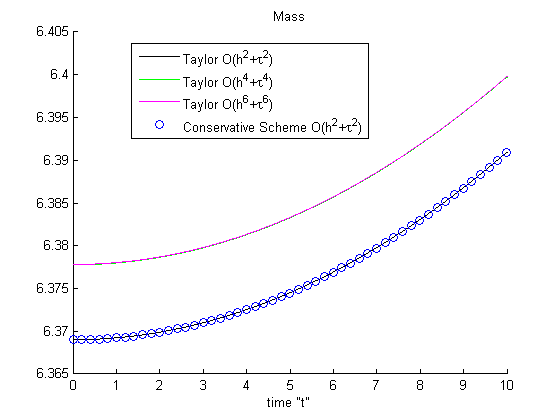
\includegraphics[width=\linewidth]{../amitans/figures/Mass_bt3_c045_h005_Taylor_Conservative.png}
	\end{minipage}	
	\begin{minipage}[b]{0.4\linewidth}
		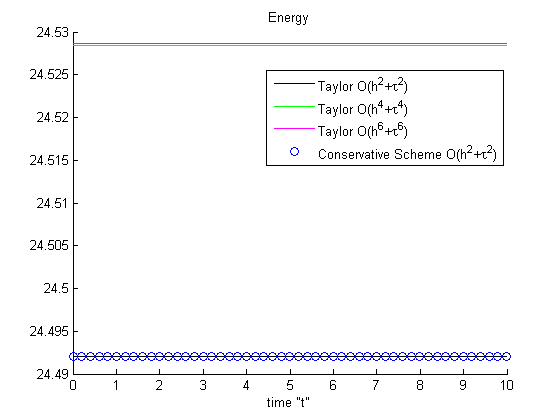
\includegraphics[width=\linewidth]{../amitans/figures/Energy_bt3_c045_h005_Taylor_Conservative.png}	
	\end{minipage}
\caption{Масата (ляво) и Енергията (дясно) на решението при Тест 1, $O(|h|^2 + \tau^2)$ и $T=10$.}
\label{Test1En}
\end{figure}
При Масата се забелязва леко покачване за целия времеви интервал $[0, T]$, но то е пренебрежимо малко спрямо началната стойност. 

При Тест 1 увеличението спрямо Масата в началния момент е $0.33\%$, а при Тест 2 е $1.8\%$.

\begin{figure}[ht]\vspace{0.2cm}
	\begin{minipage}[b]{0.4\linewidth}
		 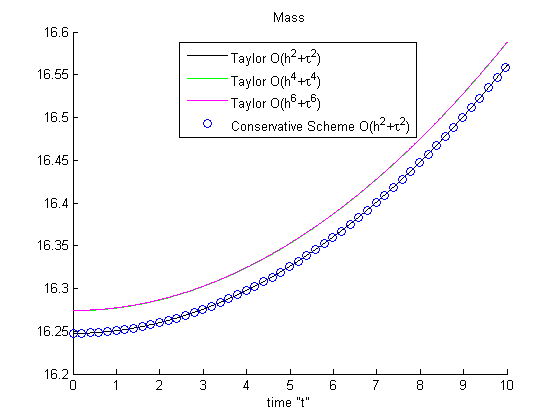
\includegraphics[width=\linewidth]{../amitans/figures/Mass_bt1_c090_h010_Taylor_Conservative.png}
	\end{minipage}	
	\begin{minipage}[b]{0.4\linewidth}
		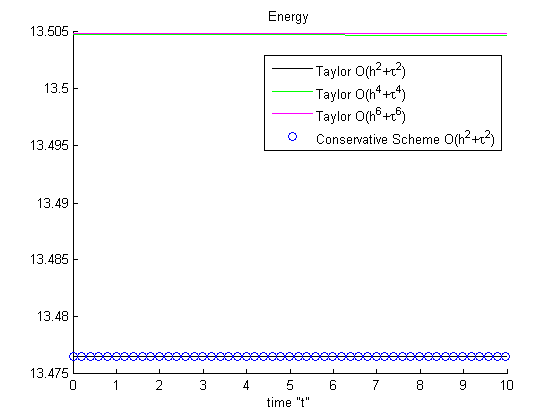
\includegraphics[width=\linewidth]{../amitans/figures/Energy_bt1_c090_h010_Taylor_Conservative.png}
		
	\end{minipage}
\caption{Масата (ляво) и Енергията (дясно) на решението при Тест 2, $O(|h|^2 + \tau^2)$ и $T=10$.}
\label{Test2En}
\end{figure}

При метода на Тейлор, дискретната Маса и Енергия показани на Фигура \ref{Test1En} са пресметнати с три различни апроксимации - правило на трапците \rf{quadr2}, правило на Симпсън \rf{quadr4} и правило на Буул \rf{quadr6-2D}, съответно с грешка от апроксимацийте $O(h^2)$, $O(h^4)$ и $O(h^6)$.  
Вижда се че с увеличаване степента на апроксимация, нарастването на масата остава непроменено. Направени са допълнителни изчисления с по-малки стъпки $h$ по пространството (графиките са изпуснати, за да не се претрупва съдържанието), което също не води до съществена промяна във функцията на Масата. Затова в по-следващите изчисления, за да се обясни нейното поведението, се използва една и съща апроксимация - $O(h^6)$ с правилото на Буул - с фиксирана стъпка по пространството $h$, а размерите на изчислителната област се увеличават.
%----------------------------------------------------------------------------------------------------------------------------------------------
\iffalse
\begin{figure}[ht]\vspace{0.4cm}
	\begin{minipage}[b]{0.33\linewidth}
		 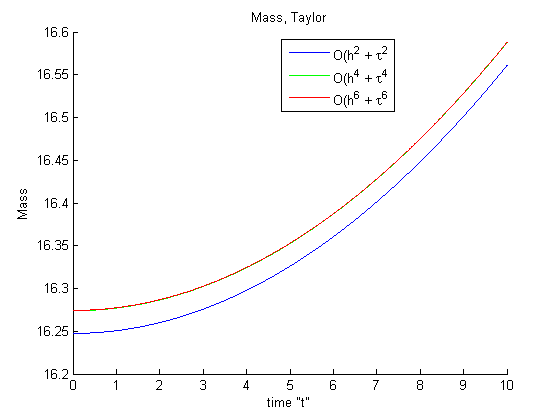
\includegraphics[width=\linewidth]{../amitans/figures/Mass_bt1_c090_h010_x3O.png}
	\end{minipage}	
	\begin{minipage}[b]{0.33\linewidth}
		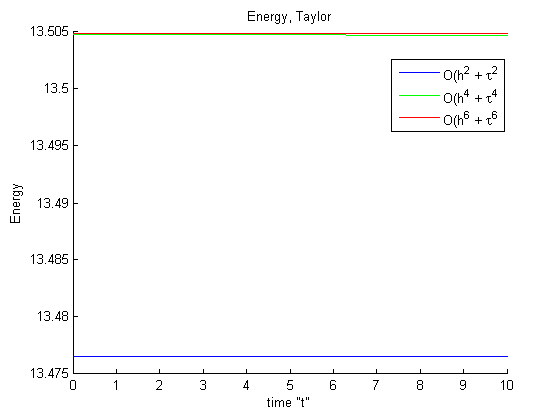
\includegraphics[width=\linewidth]{../amitans/figures/Energy_bt1_c090_h010_x3O.png}
		
	\end{minipage}
\caption{Масата (ляво) и Енергията (дясно) на решението при метода на Тейлор за Тест 1, $O(|h|^2 + \tau^2)$, $O(|h|^4 + \tau^4)$, $O(|h|^6 + \tau^6)$ и $T=10$.}
\label{Test1TEn}
\end{figure}
\begin{figure}[ht]\vspace{0.4cm}
	\begin{minipage}[b]{0.33\linewidth}
		 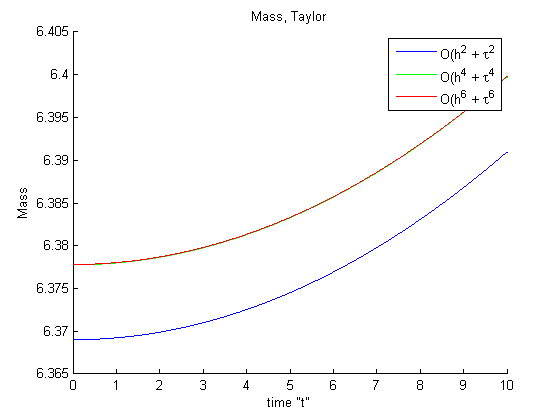
\includegraphics[width=\linewidth]{../amitans/figures/Mass_bt3_c045_h005_x3O.png}
	\end{minipage}	
	\begin{minipage}[b]{0.33\linewidth}
		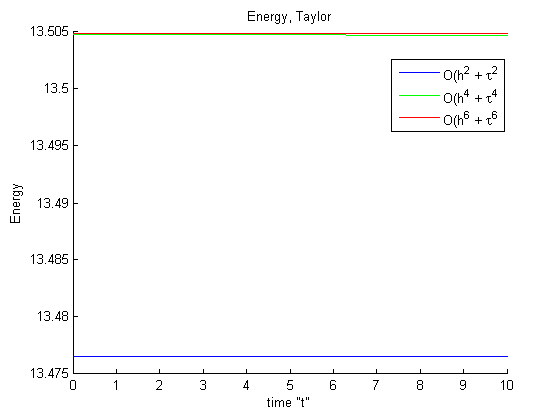
\includegraphics[width=\linewidth]{../amitans/figures/Energy_bt1_c090_h010_x3O.png}
		
	\end{minipage}
\caption{Масата (ляво) и Енергията (дясно) на решението при метода на Тейлор за Тест 2, $O(|h|^2 + \tau^2)$, $O(|h|^4 + \tau^4)$, $O(|h|^6 + \tau^6)$ и $T=10$.}
\label{Test2TEn}
\end{figure}
\fi
%----------------------------------------------------------------------------------------------------------------------------------------------
Ако с $D$ означим дискретната Маса то процентното увеличение на Масата се дефинира чрез $$100 \times |D(t=0) - D(t=T)|/D(t=0).$$ На Фигура \rf{Test1_2Mass} се вижда, че при увеличение на размерите на областта $\Omega_h$, увеличението на Масата намалява. При този числен експеримент, за генерирането на графиките, е използван метод на Тейлор с апроксимация от шести ред и най-големите стъпки по време и пространство ($h=0.2$ както при Тест 1 и $h=0.4$ както при Тест 2, а $\tau =  h/10$). На левия панел се вижда дискретната Маса изчислена върху три дискретни области съответно с големини 
\noindent 
\begin{equation*}
\begin{split}
& [-30, 30] \times [-27, 27], \nonumber\\
& [-60, 60] \times [-54, 54], \nonumber\\
& [-120, 120] \times [-108, 108] \nonumber\\
\end{split}
\end{equation*} 
\noindent 
при $\beta =  3$ и $c = 0.45$. Процентното увеличение на Масата спрямо увеличението на областта е измерено както следва $0.33\%$, $0.11\%$ и $0.06\%$. Аналогично, на десния панел, се вижда дискретната Маса изчислена върху три дискретни области с големини 
\noindent 
\begin{equation*}
\begin{split}
& [-128, 128] \times [-58, 58], \nonumber\\
& [-256, 256] \times [-116, 116], \nonumber\\
& [-512, 512] \times [-232, 232] \nonumber\\
\end{split}
\end{equation*} 
\noindent 
при $\beta =  1$ и $c = 0.9$. Тук процентното увеличение на Масата спрямо увеличението на областта е измерено както следва $1.80\%$, $0.70\%$ и $0.18\%$.
\begin{figure}[ht]\vspace{0.2cm}
	\begin{minipage}[b]{0.4\linewidth}
		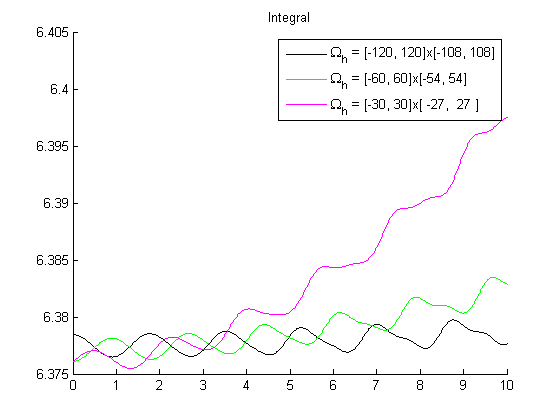
\includegraphics[width=\linewidth]{../amitans/figures/MassTaylor_120_60_30_ZB1_bt3_c045_h020_O(h^6).png}
	\end{minipage}	
	\begin{minipage}[b]{0.4\linewidth}
		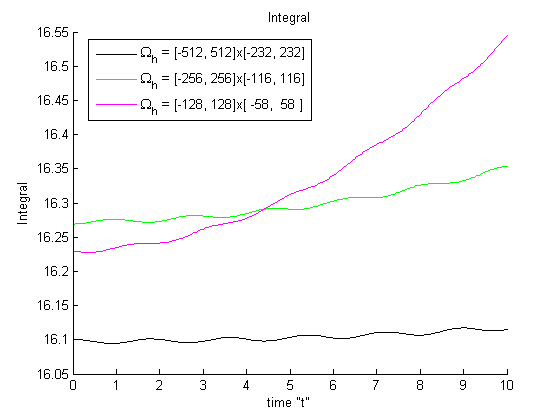
\includegraphics[width=\linewidth]{../amitans/figures/MassTaylor_512_256_128_ZB1_bt1_c090_h040_O(h^6).png}
		
	\end{minipage}
\caption{Масата от решението на Тейлор при $O(|h|^6 + \tau^6)$ апроксимация и време $T=10$ върху три различни по големина области. Левия панел е при $\beta =  3$, $c = 0.45$, а десния панел е при $\beta =  1$, $c = 0.9$.}
\label{Test1_2Mass}
\end{figure}
Тези резултати и разсъждения не доказват, че Масата е константна величина спрямо времевата променлива в непрекъсната област $\Omega$. Но въпреки това се вижда, че те не противоречат на последното твърдение, а точно обратното - подкрепят го. 

\subsection{Числени резултати за формата и максимума на решението}

В този параграф се разглежда формата на решението получена както с Консервативната схема и така и с метода на Тейлор. Стойностите на използваните параметри са описани в Таблица \ref{tableP}, когато $p=2$. Накратко, това са числени резултати от Тест 1 и Тест 2, при двата метода на решение, върху три вложени мрежи и с апроксимационни формули само от втори ред. Нека да означим с $uC$ и $uT$ двата класа от решения получени съответно с Консервативната схема \rf{consFDS} и метода на Тейлор \rf{TSe}. 
Фигури \ref{Test1_Diff} и \ref{Test2_Diff} илюстрират разликите между двата класа от решения получени съответно при Тест 1 и Тест 2. Графиките обхващат само централната (1/9) част от числената област $\Omega_h$, където отклоненията са по-големи. Ако разделим мислено $\Omega_h$ на по три равни по площ части, първо по дължина, а после и по ширина се получават девет еднакви правоъгълника като в картинките се разглежда средният.
\begin{figure}[ht]\vspace{0.4cm}
	\begin{minipage}[b]{0.32\linewidth}
		 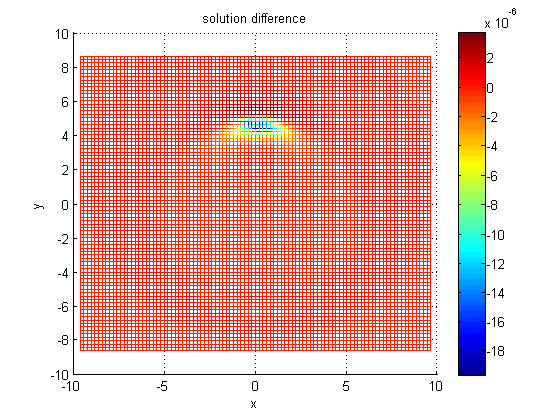
\includegraphics[width=\linewidth]{../amitans/figures/compare_30_bt3_c045_h020.png}
	\end{minipage}	
	\begin{minipage}[b]{0.32\linewidth}
		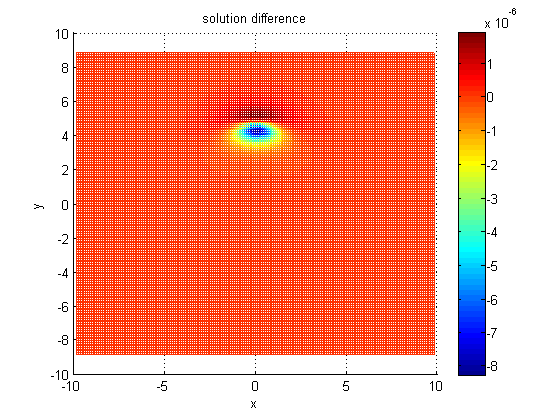
\includegraphics[width=\linewidth]{../amitans/figures/compare_30_bt3_c045_h010.png}
	\end{minipage}	
	\begin{minipage}[b]{0.32\linewidth}		
		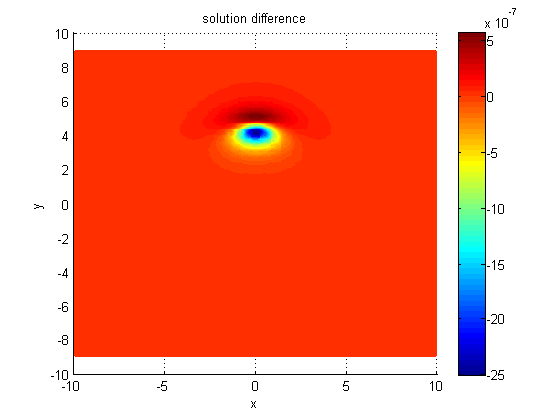
\includegraphics[width=\linewidth]{../amitans/figures/compare_30_bt3_c045_h005.png}
	\end{minipage}
\caption{Разликите $uC - uT$ между класовете от решения получени при Консервативната схема и метода на Тейлор при време $t=10$ и апроксимация $O(|h|^2 + \tau^2)$ при Тест 1. От ляво на дясно се променят стъпките както следва $h=0.2, 0.1, 0.05$.}
\label{Test1_Diff}
\end{figure}

\begin{figure}[ht]\vspace{0.4cm}
	\begin{minipage}[b]{0.32\linewidth}
		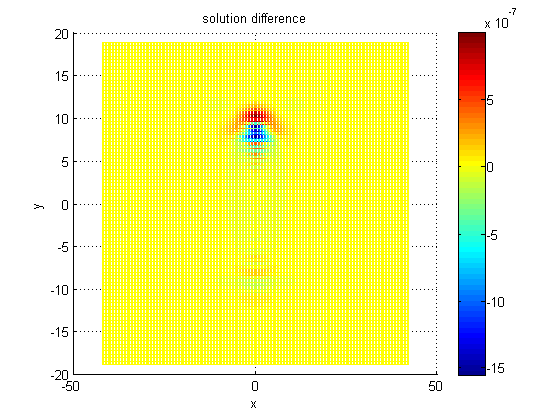
\includegraphics[width=\linewidth]{../amitans/figures/compare_128_bt1_c09_h040.png}
	\end{minipage}	
	\begin{minipage}[b]{0.32\linewidth}
		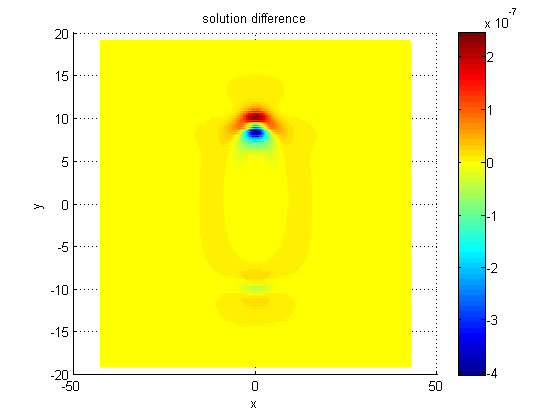
\includegraphics[width=\linewidth]{../amitans/figures/compare_128_bt1_c09_h020.png}
	\end{minipage}	
	\begin{minipage}[b]{0.32\linewidth}
		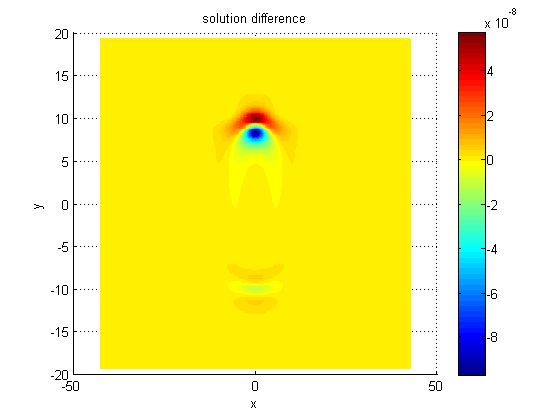
\includegraphics[width=\linewidth]{../amitans/figures/compare_128_bt1_c09_h010.png}
	\end{minipage}
\caption{Разликите $uC - uT$  между класовете от решения получени при Консервативната схема и метода на Тейлор при време $t=10$ и апроксимация $O(|h|^2 + \tau^2)$ при Тест 2. От ляво на дясно се променят стъпките както следва $h=0.4, 0.2, 0.1$.}
\label{Test2_Diff}
\end{figure}

\begin{figure}[ht]\vspace{0.2cm}
\centering
	\begin{minipage}[b]{0.30\linewidth}
		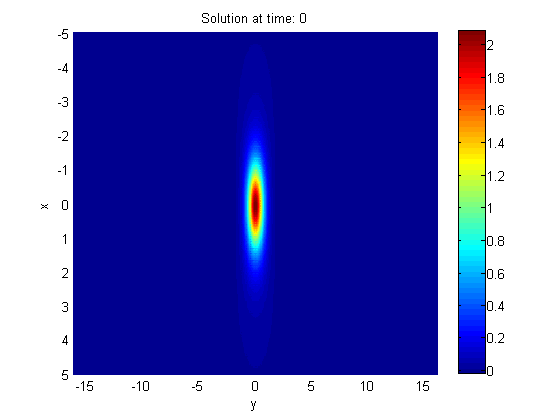
\includegraphics[width=\linewidth]{../amitans/figures/solution_30x45_bt3_c045_T0.png}
	\end{minipage}	
	\begin{minipage}[b]{0.30\linewidth}
		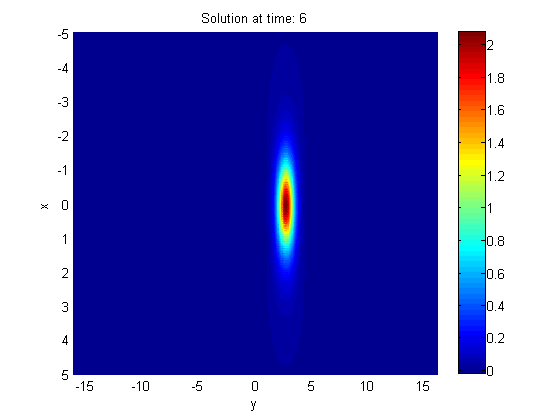
\includegraphics[width=\linewidth]{../amitans/figures/solution_30x45_bt3_c045_T6.png}
	\end{minipage}	
	\begin{minipage}[b]{0.30\linewidth}
		 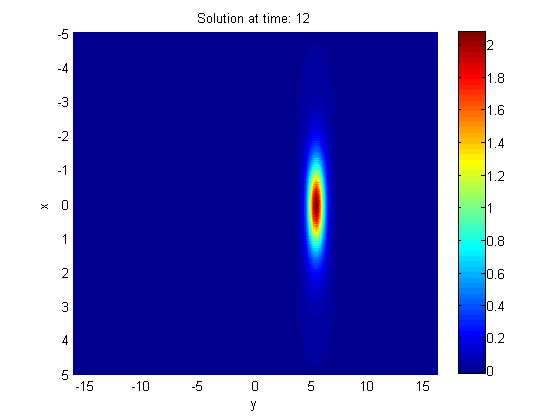
\includegraphics[width=\linewidth]{../amitans/figures/solution_30x45_bt3_c045_T12.png}
	\end{minipage}
	\begin{minipage}[b]{0.30\linewidth}
		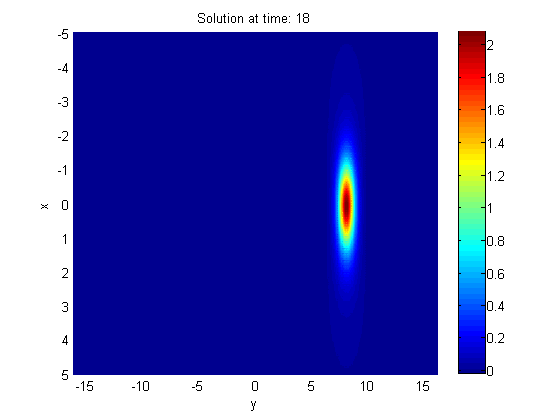
\includegraphics[width=\linewidth]{../amitans/figures/solution_30x45_bt3_c045_T18.png}
	\end{minipage}	
	\begin{minipage}[b]{0.30\linewidth}
		 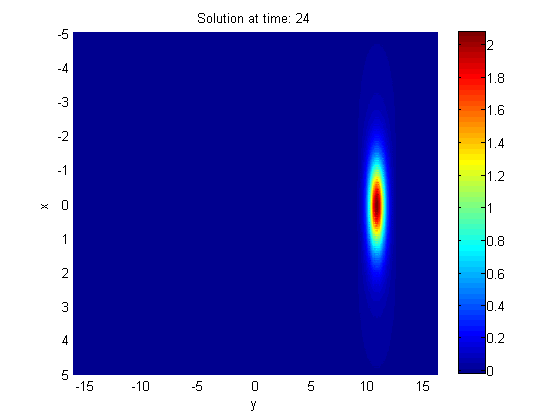
\includegraphics[width=\linewidth]{../amitans/figures/solution_30x45_bt3_c045_T24.png}
	\end{minipage}
	\begin{minipage}[b]{0.30\linewidth}
		 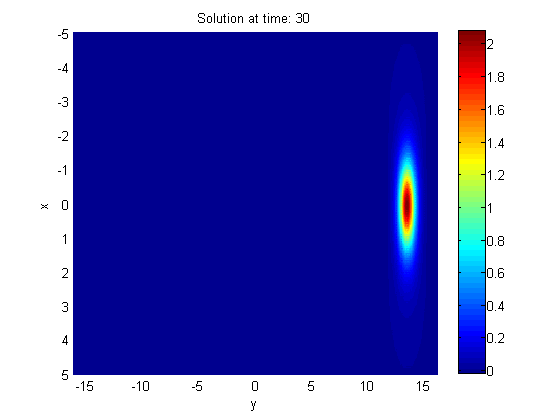
\includegraphics[width=\linewidth]{../amitans/figures/solution_30x45_bt3_c045_T30.png}
	\end{minipage}
\caption{Числени резултати за една вълна при $\beta=3$ и $c = 0.45$ за времена $t=0,6,12,18,24,30$.}
\label{Wave1}
\end{figure}

\begin{figure}[ht]\vspace{0.2cm}
\centering
	\begin{minipage}[b]{0.30\linewidth}
		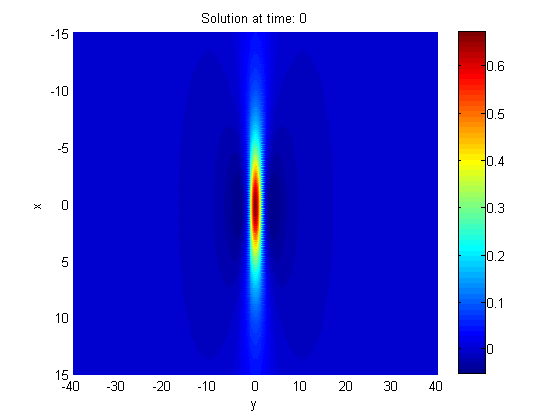
\includegraphics[width=\linewidth]{../amitans/figures/solution_128x90_bt1_c090_T0.png}
	\end{minipage}	
	\begin{minipage}[b]{0.30\linewidth}
		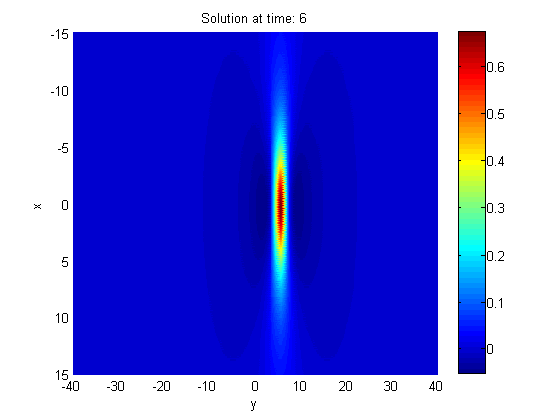
\includegraphics[width=\linewidth]{../amitans/figures/solution_128x90_bt1_c090_T6.png}
	\end{minipage}	
	\begin{minipage}[b]{0.30\linewidth}
		 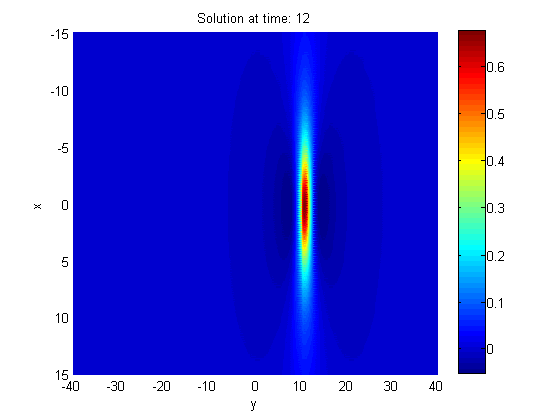
\includegraphics[width=\linewidth]{../amitans/figures/solution_128x90_bt1_c090_T12.png}
	\end{minipage}
	\begin{minipage}[b]{0.30\linewidth}
		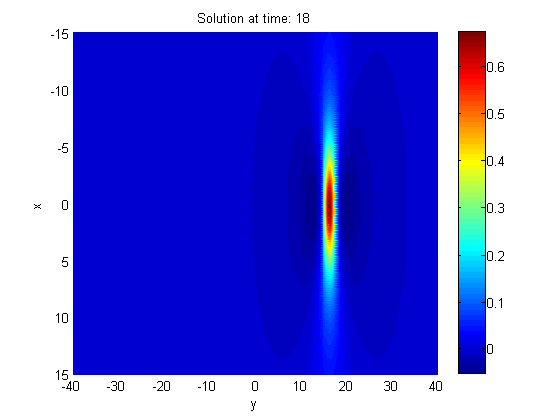
\includegraphics[width=\linewidth]{../amitans/figures/solution_128x90_bt1_c090_T18.png}
	\end{minipage}	
	\begin{minipage}[b]{0.30\linewidth}
		 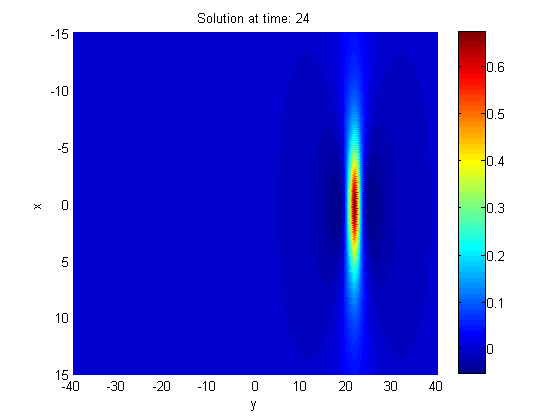
\includegraphics[width=\linewidth]{../amitans/figures/solution_128x90_bt1_c090_T24.png}
	\end{minipage}
	\begin{minipage}[b]{0.30\linewidth}
		 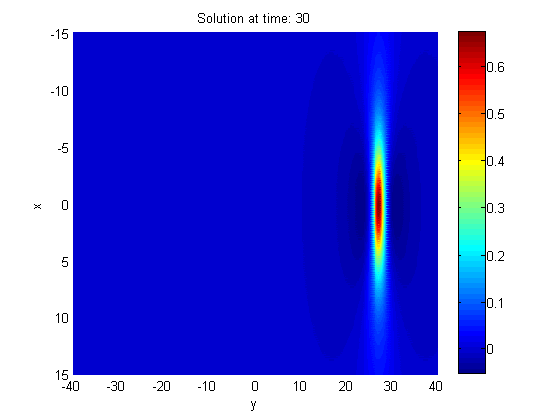
\includegraphics[width=\linewidth]{../amitans/figures/solution_128x90_bt1_c090_T30.png}
	\end{minipage}
\caption{Числени резултати за една вълна при $\beta=1$ and $c = 0.9$ за времена $t=0,6,12,18,24,30$.}
\label{Wave2}
\end{figure}

Фигурите показват, че най-големите различия се проявяват около и в максимума на вълната. В допълнение към последните резултати е Таблица \ref{tableF}, която отново показва разликите $||uC - uT||_\kappa$ в  $L_2$ и ${L_\infty}$ норми. Първата колона от таблицата е за вида на числения тест, който е направен. Във втората колона са описани стъпките по пространството и времето. В третата и четвъртата са разликите от решенията между двата метода в $L_2$ и ${L_\infty}$ норми. Последната колона от таблицата е безкрайната норма на решението (което е максимума) при Консервативната схема. Наблюдава се, че при намаляване на дискретните стъпки $h$ и $\tau$ различията стават по-малки. Също така процентната разлика между двете решения дефинирана с безкайната норма
$$\frac{ ||uC - uT||_{L_\infty}} { ||uC||_{L_\infty} } \times 100$$
варира в интервала $[0.0001\%, 0.69\%]$ за всички случаи описани в таблицата. Аналогични резултати са получени и при процентната разлика дефинирана с $L_2$ нормата и затова те са пропуснати. Формите на решенията получени с Консервативната схема и метода на Тейлор са доста близки и от числените резултати се забелязва тенденцията, че разликата $||uC - uT||_\kappa$ клони към нула когато стъпките $h$ и $\tau$ са безкрайно малки.

%F
\begin{table}[ht]
\centering
\small
		\begin{tabular}{||c|l|l|l|l||}
			\hline
			\hline
      FDS        &$h$, $\tau$  &   $||uC - uT||$  in $L_2$     &  $||uC - uT||$ in $L_\infty$ & $||uC||$ in $L_\infty$ \\
   			\hline 
					\hline 
  $\beta=3$                   &0.2, 0.001         &  1.749e-05      &  1.965e-05  & 1.315448     \\
   c=0.45                        &0.1, 0.0005        &  8.109e-06       & 8.274e-06 &  1.862688     \\
     $O(h^2 + \tau^ 2)$ &0.05, 0.00025     & 2.460e-06         &2.502e-06  &   2.013184   \\
			\hline 
			\hline 
       $\beta=1$          &0.4, 0.002        & 0.009981     & 0.004560 & 0.656747   \\
                  c=0.9      &0.2, 0.001        & 0.005047      & 0.002373  & 0.673901   \\
  $O(h^2+ \tau^2)$ &0.1, 0.0005         & 0.002521      &0.001117 & 0.672231   \\
			\hline
	   \hline
			\hline 
		\end{tabular}
		\caption{Разлики $uC - uT$ между двата класа от решения получени от Консервативната схема и метода на Тейлор при време $t=10$ а апроксимация $O(|h|^2 + \tau^2)$. Разликите са измерени в $L_2$ и $L_\infty$ норми.}
\label{tableF}
\end{table}

В този параграф се разглежда запазването на формата на решението във времевия интервал $[0, 10]$. Както и в по-горните случаи така и тук с помощта на параметричната Таблица \ref{tableP} се описват компютърните изчисления. Използван е метод на Тейлор с втори, четвърти и шести ред на апроксимация, а при всяка от апроксимациите са използвани три вложени мрежи. Резултатите са представени в Таблица \ref{tableG}. Първата колона описва вида на теста и апроксимацията. Втората колона представя стъпките по времето и пространството $h$ и $\tau$. В третата и четвъртата колони са показани разликите между решенията в началния $t=0$ и крайния  $t=10$ момент от време в  $L_2$ и $L_\infty$ норми. Вълната изминава разтояние равно на скоростта й умножена по крайното време $t=10$. В този случай максимума на решението се намира в $(0, 10 c) \in \Omega$, а в началния момент при $t=0$ максимума се намира в нулата $(0, 0) \in \Omega$. За съжаление при Тест 1, $h=0.2$ и Тест 2, $h=0.4$ максимума на решението при време $t=10$ не попада върху точка от мрежата. Затова са направени допълнителни итерации по времето с които да се отмести върха върху най-близката точка от мрежата $\Omega_h$. При Тест 1 ($c=0.45$) вълната изминава допълнително разтояние от 0.1 за време 2/9, което измества максимума в позиция $(0, 4.6) \in \Omega_h$. При Тест 2 ($c=0.9$) вълната изминава допълнително разтояние от 0.2 за време 2/9, което измества максимума в позиция $(0, 9.2) \in \Omega_h$. Разликата между двете решения $u^{(0)} - u^{(N_t)}$ може да се опише чрез матрица със следните коефициенти:
$$ \delta_{i,j} = u_{i,j}^{(0)} - u_{i,j+cT/h}^{(N_t)},$$
където $0 < i < N_x$ и $0 < j < N_y - cT/h$. 

%G
\begin{table}[ht]
\centering
\small
		\begin{tabular}{||c|l|l|l||}
			\hline
			\hline
      FDS        & $h$, $\tau$  & $||u^{(0)} - u^{(N_t)}||$ in $L_2$  & $||u^{(0)} - u^{(N_t)}||$ in $L_\infty$   \\
   		\hline 
			\hline
  $\beta=3$                &0.2, 0.001\footnote{Position of maximum is further adjusted to fit inside $\Omega_h$.}            & 1.494351 & 1.533173    \\
   c=0.45                     &0.1, 0.0005          & 0.466991 & 0.484011       \\
     $O(h^2 + \tau^ 2)$ &0.05, 0.00025   & 0.127641 & 0.132504      \\
			\hline 
  $\beta=3$               &0.2, 0.02 $^{\text{a}}$      &0.220560 & 0.230486       \\
   c=0.45                    &0.1, 0.01      &0.013762 & 0.014391        \\
     $O(h^4+ \tau^4)$ &0.05, 0.005&0.000877 & 0.000917         \\
			\hline 
  $\beta=3$               &0.2, 0.02 $^{\text{a}}$       &  0.035965 & 0.038039        \\
     c=0.45                 &0.1, 0.01        &0.000600 & 0.000633       \\
     $O(h^6+ \tau^6)$ &0.05, 0.005 &0.000010 & 0.000010          \\
	   \hline
			\hline 
       $\beta=1$       &0.4, 0.002 $^{\text{a}}$       & 0.244208 & 0.103833 \\
                  c=0.9    &0.2, 0.001       &  0.057175 & 0.026919  \\
  $O(h^2+ \tau^2)$ &0.1, 0.0005   & 0.013938 & 0.006622  \\
			\hline
      $\beta=1$               &0.4, 0.04 $^{\text{a}}$    &0.028546 & 0.012203 \\
       c=0.9                     &0.2, 0.02     & 0.001757 & 0.000958     \\
       $O(h^4+ \tau^4)$ &0.1, 0.01   & 0.000112 & 0.000061   \\
    \hline
  $\beta=1$                  &0.4, 0.04 $^{\text{a}}$   &0.006415 & 0.002792  \\
      c=0.9                    &0.2, 0.02   &0.000112 & 0.000065     \\
     $O(h^6+ \tau^6)$ &0.1, 0.01 & 0.000002 & 0.000001         \\
	   \hline
			\hline 
		\end{tabular}
		\caption{Разликата $||u^{(0)} - u^{(N_t)}||_\kappa$ в $L_2$ и $L_\infty$ норми между решенията в началния $t=0$ и крайния $t=10$ моменти от време. За резултатите от таблицата е използван единствено метода на Тейлор.}
\label{tableG}
\end{table}

Таблица \ref{tableG} показва, че с намаляване на стъпките по пространството $h$ и времето $\tau$, разликата между разгледаните решения също намалява. В допълнение се вижда, че формата на вълната се запазва по-добре, когато степента на апроксимация $p$ на диференциалните оператори е по-висока. Последните разсъждения затвърждават очакването, че разликата във формата на решението $||u^{(0)} - u^{(N_t)}||_\kappa$ при различни времена клони към нула когато $h$ и $\tau$ са безкрайно малки.

\begin{figure}\vspace{0.2cm}
	\centering
	\begin{minipage}[b]{0.40\linewidth}
		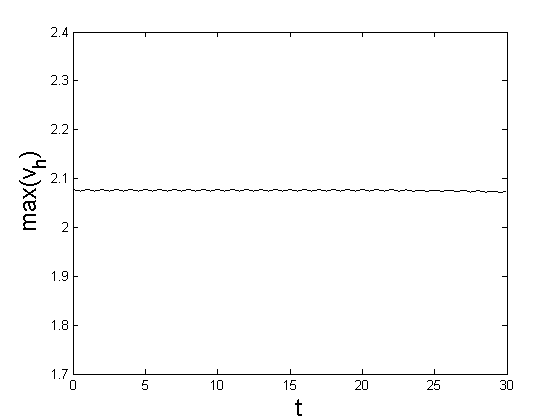
\includegraphics[width=\linewidth]{../amitans/figures/maximum_30_T30_bt3_c045_h005.png}
	\end{minipage}	
	\begin{minipage}[b]{0.40\linewidth}
		 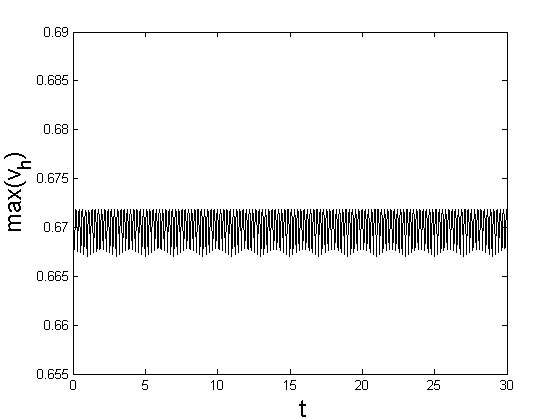
\includegraphics[width=\linewidth]{../amitans/figures/maximum_30_T30_bt1_c090_h020.png}
	\end{minipage}
\caption{Развитие на максимума на решението върху по-голям интервал от време $[0, 30]$ при Тест 1 (ляв панел) и Тест 2 (десен панел).}
\label{Maximum}
\end{figure}

В следния параграф се обръща внимание на максимума на решението, но при по-голям времеви интервал $[0, 30]$. Постановката за този числен експеримент е описана с помощта на Таблица \ref{tableP}, т.е. използван е метод на Тейлор с шести ред на апроксимация $p=6$, със стъпки $h=0.05$, $\tau = 0.001$ при Тест 1 и $h=0.2$,  $\tau=0.02$ при Test 2. Крайното време е $T=30$, а големината на областта $\Omega_h$ е увеличена по $y$ оста за да обхване преместването на вълната изцяло, т.е. $L_y = 45$ при Тест 1 и $L_y = 90$ при Тест 2. Както вече беше споменато, точната позиция на максимума не винаги лежи върху точка от мрежата $\Omega_h$. Това води до назъбване на графиките, което се забелязва по-отчетливо на десния панел при Тест 2 на Фигура \ref{Maximum}. Формите на решението са показани на Фигури \ref{Wave1} и \ref{Wave2} съответно при Тест 1 и Тест 2.

\begin{thebibliography}{99}

\bibitem{ref16} Angelow, K., Kolkovksa, N., Numercal Study of Traveling Wave Solutions to 2D Boussinesq Equation, {\it Serdica J. Computing}, \textbf{13} (2019), 1-16.

\bibitem{ref0} Boussinesq, J.V., Theorie des ondes et des remous qui se propagent le long d'un canal rectangulaire horizontal, en communiquant au liquide contenu dans ce canal des vitesses sensiblement pareilles de la surface au fond.  {\it Journal de Mathematiques Pures et Appliquees}, \textbf{17} (1872), 55-108.

\bibitem{ref21} Chertok, A., Christov, C.I., Kurganov, A., Central-Upwind Schemes for the Boussinesq Paradigm Equations,
{\it Computational Science and High Performance Computing IV, Notes Numer. Fluid Mech.}, \textbf{113} (2011), 267-281.

\bibitem{ref13}  Christou M. , Christov C.I.,
Galerkin spectral method for the 2D solitary waves of Boussinesq paradigm equation,
In: {\it Applications of Mathematics in Technical and Natural Sciences, Sozopol (Bulgaria)},
\emph{AIP Conference Proceedings}, \textbf{1186}, Issue 1 (2009), 217-225.

\bibitem{ref14}  Christou M. , Christov C.I.,
Fourier Galerkin method for 2D solitons of Boussinesq equation,
{\it Mathematics and Computers in Simulation} \textbf{74} (2007), 82-92.

\bibitem{ref1} Christov, C.I., An energy-consistent dispersive shallow-water model,  {\it Wave Motion}, \textbf{34} (2001), 161-174.

\bibitem{ref15} Christov, C.I., Choudhury, J., Perturbation solution for the 2D Boussinesq equation, {\it Mech. Res. Commun.}, \textbf{38} (2011), 274-281.

\bibitem{ref4} Christov, I., Christov, C.I., Physical dynamics of quasi-particles in nonlinear wave equations,
{\it Physics Letters A}, \textbf{372}, Issue 4 (2008),  841-848.

\bibitem{ref20} Christov, C.I., Kolkovska, N., Vasileva, D., On the Numerical Simulation of Un-
steady Solutions for the 2D Boussinesq Paragigm Equation,
{\it In: I. Dimov, S. Dimova, N. Kolkovska (Eds.), Numerical Methods and Applications 2010},
\emph{Conference Proceedings}, \textbf{6046} (2010), 386–394.

\bibitem{ref23} Dimova M., Vasileva D., Comparison of Two Numerical Approaches to Boussinesq Paradigm Equation, 
{\it Lect. Notes Comput. Sci.}, \textbf{8236} (2013), 255-262.

\bibitem{forn}
Fornberg, B., Generation of Finite Difference Formulas on Arbitrarily Spaced Grids, 
Math. Comput., 51(1988),  699 -- 706.

\bibitem{samarski} Samarskii, A., The Theory of Difference Schemes, Marcel Dekker Inc., New York, 2001.

\bibitem{ref22} Kolkovska, N., Angelow K., A Multicomponent Alternating Direction Method for Numerical Solving of Boussinesq Paradigm Equation,
In: {\it  I. Dimov, I., Farago, I., Vulkov, L. (eds.) NAA 2012},
\emph{Conference Proceedings}, \textbf{8236} (2013), 371–378.

\bibitem{ref25} Kolkovska N.,Two families of finite difference schemes for multidimensional Boussinesq paradigm equation, In:
{\it Applications of Mathematics in Technical and Natural Sciences,  Sozopol (Bulgaria)},
\emph{AIP Conference Proceedings}, \textbf{1301} (2010), 395.

\bibitem{ref260} G. H. Golub and C. F. Van Loan, Matrix Computations, 3/e, Johns Hopkins University, Press, Baltimore, 1996.

\bibitem{ref26} 
Strassen, Volker, Gaussian Elimination is not Optimal,
{\it Numer. Math.}, \textbf{13 (4)} (1969), 354–356, doi:10.1007/BF02165411. S2CID 121656251

\bibitem{ref27} Coppersmith, Don; Winograd, Shmuel., Matrix multiplication via arithmetic progressions,
{\it  Journal of Symbolic Computation}, \textbf{9 (3)} (1990), 251, doi:10.1016/S0747-7171(08)80013-2.

\bibitem{boole}
Zucker, Ruth, "Chapter 25.4.14: Numerical Interpolation, Differentiation, and Integration - Integration - Numerical Analysis". In Abramowitz, Milton; Stegun, Irene Ann (eds.). Handbook of Mathematical Functions with Formulas, Graphs, and Mathematical Tables. 
\it{Applied Mathematics Series} \textbf{55}  (1983), ISBN 978-0-486-61272-0.

\end{thebibliography}
\end{document}